\documentclass[a4paper, twoside, 12pt, openright]{report}

\usepackage{emptypage}

\def\thesistitle{Computational Exploration of the Medium-Chain Dehydrogenase / Reductase Superfamily}
\def\thesistitlemeta{Computational Exploration of the Medium-Chain Dehydrogenase/Reductase Superfamily}
\def\thesisauthor{Linus J. \"{O}stberg}

\usepackage[utf8x]{inputenc}
\usepackage[T2A,T1]{fontenc}

\usepackage{geometry}
\geometry{
 inner=30mm,
 outer=24mm,
 top=20mm,
 bottom=22mm
 }

 \usepackage{fancyhdr}
\fancyhf{}
\fancyfoot[LE,RO]{\thepage}
\pagestyle{fancy}
\renewcommand{\headrulewidth}{0pt} 
\fancypagestyle{plain}{
  \fancyhf{}
  \renewcommand{\headrulewidth}{0pt}
  \fancyfoot[LE,RO]{\thepage}
}

\usepackage{nomencl}
\renewcommand{\nomname}{List of Abbreviations}
\renewcommand{\nomlabel}[1]{\textbf{#1}}
\renewcommand{\nompreamble}{\thispagestyle{empty}}

\usepackage{amssymb}

\usepackage[numbib,nottoc]{tocbibind}

\usepackage{hyperref}

\usepackage{tabularx}

\newcommand{\refpaper}[1]{$^{\text{\ref{#1}}}$}

\usepackage[russian,swedish,english]{babel}
\usepackage{times}
\usepackage{csquotes}
\usepackage{graphicx}
\usepackage{color}
\usepackage{amsmath}
\usepackage{eufrak}
\usepackage[font={small}]{caption}
\usepackage[export]{adjustbox}
\usepackage{wrapfig}

\usepackage{floatrow}

\usepackage{caption}
\captionsetup{margin=10pt,font=small,labelfont=bf,singlelinecheck=false}

\usepackage{tocloft}
\renewcommand{\cfttoctitlefont}{\normalfont\LARGE\bfseries\MakeUppercase}

\usepackage{titlesec}
\usepackage{lipsum}
\titleformat{\section}{\normalfont\Large\bfseries\scshape}{\thesection}{1em}{}

\titleformat{\chapter}{\normalfont\LARGE\bfseries\scshape}{\thechapter}{20pt}{}

\AtBeginDocument{\renewcommand{\bibname}{References}}
\usepackage[super,comma,sort&compress]{natbib}
\makeatletter
\renewcommand\@biblabel[1]{#1.} % 1. i referenser
\makeatother

\usepackage{booktabs}

\usepackage{pdfpages}

\usepackage{calc}
\usepackage{enumitem}
\SetLabelAlign{parright}{\parbox[t]{\labelwidth}{\raggedleft#1}}

\usepackage{textcomp}

\usepackage{url}
\urlstyle{rm}
\usepackage{color}
\usepackage{hyperref}
\definecolor{kiplommon}{RGB}{135,0,82}
\definecolor{kicyklamen}{RGB}{212,9,99}
\hypersetup{
    colorlinks=false,
    linkcolor=kicyklamen,
    citecolor=kiplommon,
    filecolor=magenta,
    urlcolor=kiplommon,
    pdfauthor={\thesisauthor},
    pdftitle={\thesistitlemeta},
    pdfsubject={Bioinformatics, proteins},
    pdfkeywords={Medium-chain Dehydrogenase/Reductase, Alcohol Dehydrogenase, Bioinformatics, Molecular Mechanics},
    pdfproducer={TeX Live/LaTeX},
    pdfcreator={TeX Live/pdflatex}
}

\makenomenclature

\begin{document}

\pagenumbering{roman}
  
\begin{titlepage}
\newgeometry{
 inner=30mm,
 outer=24mm,
 top=30mm,
 bottom=20mm
 }


  \centering
  {\Large From the Department of Medical Biochemistry and Biophysics\\
  Karolinska Institutet, Stockholm, Sweden\par}
  \vspace{2.5cm}
  {\bfseries\LARGE \MakeUppercase{\thesistitle}\par}
  \vspace{1.5cm}
  {\large Linus J. Östberg\par}
  \vspace{3cm}
  
\includegraphics[width=0.69\textwidth]{fig/ki-logo_pos.eps}\par\vspace{1cm}

  \vspace{1.5cm}

  {\large Stockholm 2017\par}
  
  \thispagestyle{empty}

  \restoregeometry
\end{titlepage}

\newgeometry{
 inner=20mm,
 outer=24mm,
 top=20mm,
 bottom=60mm
 }

\vspace*{\fill}

\noindent All previously published papers were reproduced with permission from the publisher.

\noindent Published by Karolinska Institutet.

\noindent Printed by E-Print AB 2017

\noindent \textcopyright \thesisauthor, 2017

\noindent ISBN 978-91-7676-650-7
\thispagestyle{empty}

\newpage

\restoregeometry

\newgeometry{
 inner=30mm,
 outer=24mm,
 top=30mm,
 bottom=20mm
 }

{\Large \noindent \MakeUppercase{\thesistitle}\par}
\vspace{0.5cm}
{\Large \noindent THESIS FOR DOCTORAL DEGREE (Ph.D.) \par}
\vspace{0.5cm}
{\noindent By \par}
\vspace{0.5cm}
{\Large \noindent \bf \thesisauthor\par}
\vspace{0.5cm}

{\small
\begin{flushleft}
\begin{tabularx}{\textwidth}{lXl}
{\em Principal Supervisor:} & & {\em Opponent:}\\
Prof. Jan-Olov Höög & & Prof. Jaume Farrés\\
Karolinska Institutet & & Autonomous University of Barcelona\\
Department of Medical Biochemistry and & & Department of Biochemistry and \\
Biophysics & & Molecular Biology\\
\\
{\em Co-supervisor:} & & {\em Examination Board:}\\
Prof. Bengt Persson & & Prof. Erik Lindahl\\
Uppsala University & & Stockholm University\\
Department of Cell and Molecular Biology & & Department of Biochemistry and Biophysics\\
\\
& & Assoc. Prof. Tanja Slotte\\
& & Stockholm University\\
& & Department of Ecology, Environment \\
& & and Plant Sciences\\
\\
& & Prof. Elias Arnér\\
& & Karolinska Institutet\\
& & Department of Medical Biochemistry and\\
& & Biophysics\\
\end{tabularx}
\end{flushleft}
}

\thispagestyle{empty}

\restoregeometry

\chapter*{Abstract}

The medium-chain dehydrogenase/reductase (MDR) superfamily is a protein family with more than 170,000 members across all phylogenetic branches. In humans there are 18 representatives. The entire MDR superfamily contains many protein families such as alcohol dehydrogenase, which in mammals is in turn divided into six classes, class I--VI (ADH1--6). Most MDRs have enzymatical functions, catalysing the conversion of alcohols to aldehyde/ketones and vice versa, but the function of some members is still unknown.

In the first project, a methodology for identifying and automating the classification of mammalian ADHs was developed using BLAST for identification and class-specific hidden Markov models were generated for identification.  By using the developed methodology, multiple new mammalian ADH members were identified. Finally, the generation of a phylogenetic tree of the sequences showed the existence of a sixth class, ADH6, in most non-primate mammals, though the sequences are commonly misclassified as ADH5 or ADH1-like in the sequence databases.

The second project focused on the study of mammalian ADH5, which has never been isolated as a native protein, and whose function is unknown. The first part of the project was the expression of ADH5 fusion proteins in {\em E. coli} and COS cells (human ADH5 with glutathione-S-transferase in {\em E. coli} and rat ADH5-green fluorescent protein in COS cells). The proteins were expressed, but had no activity with any traditional ADH substrates. The results also indicated potential problems with the stability of the protein.

The continuation of the project was the analysis of the structure using computational methods. A structural model of ADH5 was generated using the homolog ADH1C as template. Molecular dynamics was subsequently used to study the properties of the model. Along with the structural analysis, extensive sequence analysis was also performed, identifying multiple positions that were unique for AHD5, e.g. Lys51 at the active site and Gly305 in the dimer-interacting region, which replace a highly conserved Pro found in ADH1--4. The combination of the structural simulations and the sequence analysis led to the conclusion that the lack of success in the isolation of ADH5 could potentially be explained by instabilities in the region involved in dimer formation, preventing the formation of the active dimers found in other ADHs. The function of ADH5 is therefore concluded to be different than that of other ADHs, but is as of yet still unknown.

The final project focused on the study of a set of human MDRs, using a combination of analyses of the structures and sequences, leading to the development of theoretical models of the binding pockets in each of the proteins, pinpointing the important residues. The positions identified to be involved in the binding of the coenzyme NADP(H) were similar between the proteins and matched currently available information in the databases, as well as further residues. The residues involved in the binding of substrates varied between the proteins, and the analysis led to the identification of three different types of substrate binding.

\thispagestyle{empty}


\chapter*{Popular Science Summary}

Back in 2003, the human genome was finally sequenced. With all this information in hand, we know the basic code for how humans work. Now we need to understand it.

The genome (the DNA) encodes proteins, which in turn build up the major part of our bodies, from the smallest strand of hair to our brains. We know how many of these proteins work, but at the same time there are many others for which we do not know the function.

The work presented in this thesis focuses on the medium-chain dehydrogenase/reductase (MDR) proteins, which form a large family of enzymes that is represented by 18 different members in humans. The function of many of these proteins are known, but the function of some of them still needs to be investigated.

Two of the projects presented here focus on the functions of the alcohol dehydrogenase (ADH) protein family, which is part of the MDR family and correspond to seven of the 18 human MDR members. As the name implies, the ADHs functions on alcohols, changing them to aldehydes, and the family also includes the enzyme responsible for the breakdown of ethanol to acetaldehyde.

The first project is focused on the classification (naming) of the mammalian ADH members (paper \ref{paper:mammalian_adhs}). In humans, only five of the six ADH classes are present, and they function on different alcohols. In the databases containing protein sequences, the classification of them is not always matching reality, and the project developed a methodology to identify ADHs in the databases and confirm (or fix) their name to match the correct class. As the methodology that was developed also led to the gathering of a high number of mammalian ADHs, it was also possible to do some comparisons between the different species, e.g. which species had which classes of ADH.

\thispagestyle{empty}

The second project focused on the analysis of the class V ADH, ADH5 (paper \ref{paper:adh5_2013} and \ref{paper:adh5_2016}). The function of ADH5 is, as opposed to the other ADHs found in humans, unknown, and nobody has ever been able to study the protein in a lab. In the first part, an attempt was made to isolate and study ADH5 by merging ADH5 with other proteins, first glutathione-S-transferase and then green fluorescent protein. The merged proteins could be isolated, but they did not act on any of the expected molecules (that are known to work with the other ADHs). It was also impossible to isolate the proteins without the extra part that had been added.

In the second part, the focus was on using bioinformatics (computational methods) to simulate and analyse the properties of ADH5. A model of the structure was made using the other human ADHs as templates, and then the model was analysed using molecular dynamics (a method that simulates the movements of the atoms over time). Along with this, the method from the first project was used to identify the sequence of the ADH5 protein in as many mammals as possible. By studying the sequences and the simulations, it was seen that ADH5 without a doubt is related to the other ADHs, but is a bit of an odd sibling. At many positions where the other ADHs had the same amino acid, ADH5 sometimes had something else. It was also seen that the structure of ADH5 was not behaving in the same way as the other ADHs. As such, it probably has a function which is different (but potentially related) to that of the other ADHs.

The final project (paper \ref{paper:mdrs}) focused on nine other human MDRs that were not part of the ADH protein family. The aim was to analyse the proteins, with focus on the area where they bind other molecules in order to modify them. The nine proteins were studied by identifying sequences in a similar way to what was used to find ADHs in the first project, followed by a sequence analysis similar to what was used to study ADH5, and finally some new ways of analysis as well. From these analyses, it could be seen that the non-ADH MDRs have at least three different types of substrate binding (where the modification of other molecules occur), using different amino acids for their effects. Further, it could be seen that NADP(H), which is used as a coenzyme (helper molecule for the enzyme) to do the modifications to other molecules) binds in a very similar way in all nine MDRs.

\thispagestyle{empty}


\chapter*{List Of Publications}

\thispagestyle{empty}

\begin{enumerate}[label=\Roman*]
 \item {\bf Östberg LJ}, Strömberg P, Hedberg JJ, Persson B, Höög J-O. Analysis of mammalian alcohol dehydrogenase 5 (ADH5): Characterisation of rat ADH5 with comparisons to the corresponding human variant. Chem Biol Interact. 2013;202(1--3):97--103.
 \label{paper:adh5_2013}
 \item {\bf Östberg LJ}, Persson B, Höög J-O. The mammalian alcohol dehydrogenase genome shows several gene duplications and gene losses resulting in a large set of different enzymes including pseudoenzymes. Chem Biol Interact. 2015;234:80--84.
 \label{paper:mammalian_adhs}
 \item {\bf Östberg LJ}, Persson B, Höög J-O. Computational studies of human class V alcohol dehydrogenase --- the odd sibling. BMC Biochem. 2016;17(1):16.
 \label{paper:adh5_2016}
 \item {\bf Östberg LJ}, Höög J-O, Persson B. Computational analysis of human medium-chain dehydrogenase/reductase revealing substrate- and coenzyme-binding characteristics. Manuscript.
 \label{paper:mdrs}
\end{enumerate}

{\let\cleardoublepage\clearpage
\chapter*{Publications Not Included in This Thesis:}

\begin{enumerate}[label=(\Alph*)]
 \item Hellgren M, Carlsson J, {\bf Östberg LJ}, Staab CA, Persson B, Höög J-O. Enrichment of ligands with molecular dockings and subsequent characterization for human alcohol dehydrogenase 3. Cell. Mol. Life. Sci. 2010;67(17):3005--3015.
 \item Höög J-O, {\bf Östberg LJ}. Mammalian alcohol dehydrogenases--a comparative investigation at gene and protein levels. Chem Biol Interact. 2011;191(1--3):2--7.
 \item Landreh M, {\bf Östberg LJ}, Pettersson TM, Jörnvall H. Transthyretin microheterogeneity and molecular interactions: implications for amyloid formation. Biomol Conc. 2014;5(3):257--264.
 \item Landreh M, {\bf Östberg LJ}, Jörnvall H. A subdivided molecular architecture with separate features and stepwise emergence among proinsulin C-peptides. Biochem Biophys Res Comm. 2014;450(4):1433--1438.
 \item Jörnvall H, Landreh M, {\bf Östberg LJ}. Alcohol dehydrogenase, SDR and MDR structural stages, present update and altered era. Chem Biol Interact. 2015;234:75--79
 \item Barbaro M, Soardi FC, {\bf Östberg LJ}, Persson B, De Mello MP, Wedell A, Lajic S. In vitro functional studies of rare CYP21A2 mutations and establishment of an activity gradient for nonclassic mutations improve phenotype predictions in congenital adrenal hyperplasia. Clinical endocrinology 2015;82(1):37--44.
 \item de Paula Michelatto D, Karlsson L, Lusa AL, Silva CD, {\bf Östberg LJ}, Persson B, Guerra-Júnior G, de Lemos-Marini SH, Barbaro M, de Mello MP, Lajic S. Functional and Structural Consequences of Nine CYP21A2 Mutations Ranging from Very Mild to Severe Effects. Int J Endocrinol. 2016;2016:4209670.
\end{enumerate}

\thispagestyle{empty}
}
\newpage

\tableofcontents

\thispagestyle{empty}

{\let\cleardoublepage\clearpage
\printnomenclature
\thispagestyle{empty}
}

\chapter{Introduction}

\pagenumbering{arabic}

\begin{figure}[h]
 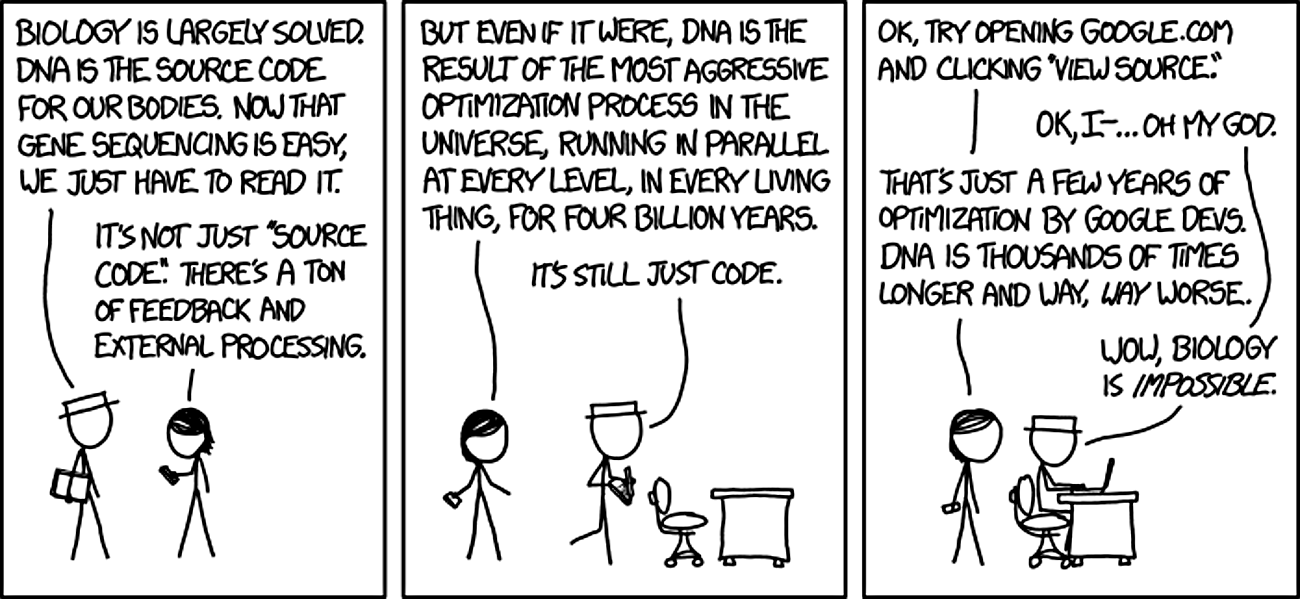
\includegraphics[width=0.9\textwidth]{fig/xkcd_dna.png}
 \caption{xkcd: DNA\cite{munroe_xkcd_2017} / \href{https://creativecommons.org/licenses/by-nc/2.5/}{CC BY-NC 2.5}}
\end{figure}

As defined by the central dogma of molecular biology\cite{crick_central_1970}, DNA is transcribed into RNA, which in turn is translated into proteins. This means that DNA is used to store the genetic information in the chromosomes. The DNA can be transcribed to multiple copies of RNA as a means to control the expression, and finally each mRNA can be translated into multiple copies of the same protein. The various functions that are needed within an organism are performed by the proteins (and to a minor part, the RNA). As such, the understanding of the function of each protein is essential to fully understand the molecular function of an organism.


\section{Bioinformatics}

Traditionally, biomedical processes have been studied using biochemical and biophysical methods. As the knowledge in the field of biochemistry increased, the field of bioinformatics appeared in the 1970s with the goal of making theoretical models that would fit biological data, intended to follow the concept of ``theoretical biology''\cite{hogeweg_roots_2011}.

Over time, the biochemical methodologies improved, generating more and more data, especially with the advent of high-throughput methods such as next-generation sequencing. In 2003, the sequencing of the human genome was a major milestone\cite{the_international_human_genome_sequencing_consortium_international_2003}, but in 2017, the sequencing of human genomes is done routinely. Similar improvements can be seen in other biochemical fields, including mass spectrometry, structural biology, expression analysis, and many others.

As an effect of the greater amounts of generated data, the definition of the field of bioinformatics transformed, from the original definition of making theoretical models, to being more about analysing biological data. The field of bioinformatics today covers many areas, including DNA and RNA sequence analysis, protein sequence analysis, phylogeny, structural biology, and systems biology. It also includes the prediction and simulation of different biomedical properties, e.g. calculating structural models of proteins.

The fields of biochemistry and bioinformatics now work in unison, the biochemical methods generating data, which can be evaluated and used for further analysis by the bioinformatics methods.

Along with the generation of scientific data, there is also the need to store the data and to make it available to other researchers.

One of the earliest ``systems'' for the publication of sequence data was Dayhoff's Atlas of Protein Sequence and Structure, which in 1969 reported all (initially 65) protein sequences that were known at the time\cite{dayhoff_atlas_1969}. It was printed as multiple volumes, and led to the development of the Protein Information Resource\cite{wu_protein_2003} (PIR), \nomenclature{PIR}{Protein Information Resource} the first protein sequence database accessible by remote computers. 

After PIR came more sequence databases. Originally the development efforts were done independently, causing USA, Europe, and Japan to have their own sequence databases. Over time, they started collaborating, and while each site still runs their own databases, the sequence data is now being synchronised. Though the sequences are shared, each site still maintain their own systems with unique user interfaces.


\section{Medium-chain Dehydrogenase/Reductase}
\label{sec:mdr}

The medium-chain dehydrogenase/reductase (MDR) \nomenclature{MDR}{Medium-chain dehydrogenase/reductase} superfamily is a protein family with a large number of member proteins, both from eukaryotes and prokaryotes. Due to the large number of members, it is often referred to as a superfamily, its members in turn forming protein families of their own\cite{persson_super-family_1994}.

The first characterised MDR member was alcohol dehydrogenase, which sequence from horse liver class I \nomenclature{ADH}{Alcohol dehydrogenase} was determined in 1970 \cite{jornvall_horse_1970-1}. After the initial member was found, more members were discovered, and the name of the of the superfamily, MDR, was termed to separate the MDRs from another protein family with similar function, the short-chain dehydrogenase/reductase (SDR) \nomenclature{SDR}{Short-chain dehydrogenase/reductase} superfamily \cite{persson_characteristics_1991}. The MDRs generally have $\sim$350 amino acid residues per subunit (though there are exceptions) while the SDRs generally have $\sim$250 amino acid residues\cite{persson_characteristics_1991}.
 
The MDR superfamily has considerable multiplicity, with 18 human family members, including the alcohol dehydrogenases (ADH; EC 1.1.1.1), prostaglandin reductases (PTGR; 1.3.1.48), \nomenclature{PTGR}{Prostaglandin reductase} quinone oxidoreductases (QOR; EC 1.3.1.27), \nomenclature{QOR}{Quinone oxidoreductase} sorbitol dehydrogenases (SORD; EC 1.1.1.14), \nomenclature{SORD}{Sorbitol dehydrogenase} as well as multiple other enzymes (Table \ref{table:human_mdrs}). The number of proteins increases as more species are analysed. Multiple attempts to classify the family have been made. One such separated the 15,000 sequences known in 2010 into 86 unique clusters with at least 20 protein sequences each\cite{hedlund_subdivision_2010}, and a large number of small clusters with fewer member that were not evaluated at the time. The total number of unique families has been estimated to $\sim$500 with $\sim$30\% sequence identify between the families\cite{persson_medium-_2008}.

\begin{table}[htb]
\begin{center}
\ttabbox[\FBwidth]
{\caption{Human MDR members, using UniProtKB/Swiss-Prot annotations.}
\label{table:human_mdrs}}
{\begin{tabular}{lllll}
\toprule
Protein name & Gene & UniProt & Structure$^1$ & Coenzyme\\
\midrule
Alcohol dehydrogenase 1A & ADH1A & P07327 & 1U3T (2) & NAD(H)\\
Alcohol dehydrogenase 1B & ADH1B & P00325 & 1U3V (9) & NAD(H)\\
Alcohol dehydrogenase 1C & ADH1C & P00326 & 1U3W (3) & NAD(H)\\
Alcohol dehydrogenase 4 & ADH4 & P08319 & 3COS (1) & NAD(H)\\
Alcohol dehydrogenase 6 & ADH6 & P28332 & Unknown & Unknown\\
Alcohol dehydrogenase class-3 & ADH5 & P11766 & 2FZW (9) & NAD(H)\\
Alcohol dehydrogenase class 4 & ADH7 & P40394 & 1D1T (3) & NAD(H)\\
mu/sigma chain\\
Enoyl-[acyl-carrier-protein] & MECR & Q9BV79 & 1ZSY (2) & NADP(H)\\
reductase, mitochondrial\\
Fatty acid synthase & FASN & P49327 & 3TJM (12) & NADP(H)\\
Prostaglandin reductase 1 & PTGR1 & Q14914 & 2Y05 (2) & NADP(H)\\
Prostaglandin reductase 2 & PTGR2 & Q8N8N7 & 2ZB4 (6) & NADP(H)\\
Prostaglandin reductase 3 & PTGR3 & Q8N4Q0 & 2C0C (4) & NADP(H)\\
Quinone oxidoreductase & CRYZ & Q08257 & 1YB5 (1) & NADP(H)\\
Quinone oxidoreductase PIG3 & TP53I3 & Q53FA7 & 2J8Z (2) & NADP(H)\\
Reticulon-4-interacting protein 1, & RTN4IP1 & Q8WWV3 & 2VN8 (1) & NADP(H)\\
mitochondrial\\
Sorbitol dehydrogenase & SORD & Q00796 & 1PL8 (3) & NAD(H)\\
Synaptic vesicle membrane protein & VAT1 & Q99536 & Unknown & Unknown\\
VAT-1 homolog\\
Synaptic vesicle membrane protein & VAT1L & Q9HCJ6 & 4A27 (1) & NADP(H)\\
VAT-1 homolog-like\\
\bottomrule
\\[-10pt]
\multicolumn{5}{l}{$^1$PDB code of one structure (total number of structures in PDB)}
\end{tabular}}
\end{center}
\end{table}

There are three domain definitions of the MDR proteins in Pfam\cite{finn_pfam:_2014}, each covering different members and parts of the proteins; ADH$\_$N (Alcohol dehydrogenase GroES-like domain; PF08240), ADH$\_$N$\_$2 (N-terminal domain of oxidoreductase; PF16884), and ADH$\_$zinc$\_$N (Zinc-binding dehydrogenase; PF00107). Together, the definitions identify, as of February 2017, more than 170,000 MDR proteins in the UniProt sequence database\refpaper{paper:mdrs}, a number that increases with each new release of the database.


\subsection{Structure}

The structure of an MDR protein is formed by two domains; one C-terminal coenzyme (NAD(H)/NADP(H)) binding domain with the common Rossmann fold \cite{rao_comparison_1973}; typically six $\beta$-strands forming a $\beta$-sheet with $\alpha$-helices above and below, and one substrate-binding domain consisting of antiparallel $\beta$-strands with $\alpha$-helices at the surface, similar to the GroES fold \cite{taneja_conserved_1999}, the binding pocket being located inside the cleft between the two domains. 

MDRs often form homodimers, but both monomeric (e.g. mannitol dehydrogenase\cite{stoop_purification_1995}) and tetrameric (e.g. yeast alcohol dehydrogenase I\cite{raj_yeast_2014}) members are known to exist.

Currently, for 61 of the MDR proteins listed in UniProtKB/Swiss-Prot, there is an X-ray crystal structure is available, and the number is increased to 117 if the proteins in UniProtKB/TrEMBL are also included. Of these 117 proteins, 16 are the human forms, meaning that the structures are still unknown for only two human MDR proteins. It also means that a majority of all known MDRs does not have known structure, though many are expected to be homologous to the known structures. 
  
 \begin{figure}[htbp]
   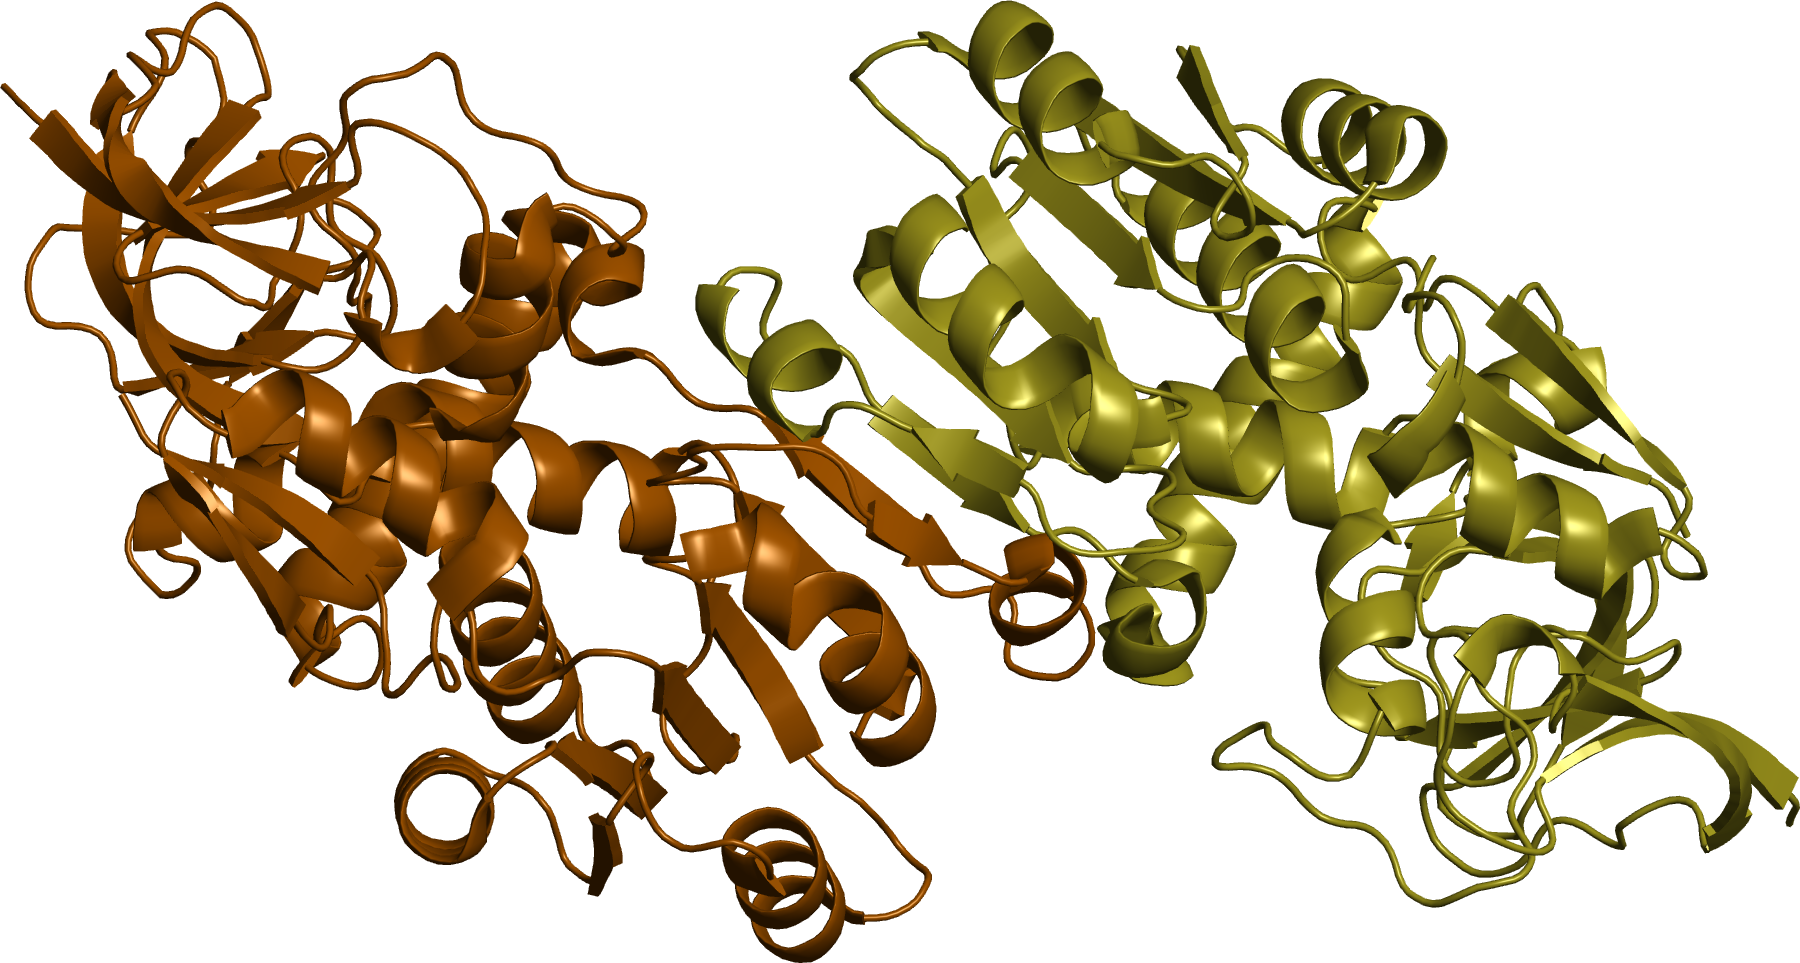
\includegraphics[width=0.9\textwidth]{fig/mdr_structure.png}
  \caption{Typical dimeric MDR structure: human QOR (PDB id: 1YB5).}
  \label{fig:mdr_structure}
 \end{figure}


\subsection{Function}

As there are a multitude of different MDRs, there is also a large variety of functions. The characterised MDR members generally function as enzymes catalysing the reaction Alcohol + NAD(P)$^+$ $\rightleftarrows$ Aldehyde/ketone + NAD(P)H, where the enzymes using NAD$^+$  typically function as dehydrogenases, while the ones using NADPH function as reductases\cite{persson_medium-_2008}. Though the function of many MDR members are known, there are many more with unknown function.

The MDRs are homologs, though their sequences show a great level of variation, but the proteins all share similar folds. However, the binding pockets can vary quite a bit. The mammalian alcohol and sorbitol dehydrogenases use Zn$^{2+}$ ions to help with the coordination of the substrates\cite{jornvall_alcohol_1981}, while many other MDRs use Tyr\cite{porte_three-dimensional_2009}. There are different types of binding pockets among the proteins using Tyr, each containing the Tyr at different positions, and some including a second Tyr\refpaper{paper:mdrs}.

The substrate specificities vary greatly among the MDRs, from ethanol\cite{hoog_mammalian_2001-1} to benzoquinone\cite{hoog_mammalian_2001-1}, prostaglandins\cite{wu_structural_2008}, fatty acids\cite{jayakumar_human_1995}, and trans-2-hexenoyl-CoA\cite{miinalainen_characterization_2003}.


\subsection{Alcohol Dehydrogenase}
\label{sec:adh}

Alcohol dehydrogenase is the largest of the MDR families. In the 2010 classification of MDRs\cite{hedlund_subdivision_2010}, there were more than 2200 sequences in the main cluster, as well as hundreds in smaller clusters. As the total number of MDR sequences since then has grown by an order of magnitude, the number of ADH sequences are expected to have increased by a considerable amount as well.

There are multiple isoforms, classes, present in different species. In mammals, there are six classes, class I--VI (ADH1--6) with $\sim$60\% sequence identity between the classes. The classes is a common source of confusion, as the numbering is based on the order of discovery, and the proteins and the genes do not necessarily have the same number. This thesis uses the classification recommended in 1999\cite{duester_recommended_1999}, where the class I ADH is annotated as ADH1, class II as ADH2, and so forth. In humans, there are seven ADH genes, corresponding to ADH1--5\cite{hoog_mammalian_2001-1, jornvall_alcohol_2015}, with three isoforms of ADH1\cite{vallee_isozymes_1983} (Table \ref{table:adh_nomenclature}).

The human ADHs are mainly expressed in the liver, but may be found in varying amounts in other tissues as well. The exceptions are ADH3 which can be found in most tissues, and ADH4 which is not found in the liver, but in the stomach and the intestines\cite{estonius_alcohol_1996}.

The substrate specificities of the classes vary. The ADH1 isoforms are the traditional enzymes involved in the breakdown of ethanol to acetaldehyde, but also have activity with e.g. retinol, hydroxysteroids, and hydroxytryptophol. ADH2 has a high activity with ethanol, but with a high K$_m$\cite{hoog_mammalian_2001-1}. The preferred substrates are retinol\cite{hellgren_alcohol_2007} and benzoquinone\cite{svensson_structural_1998}. ADH3 acts especially on S-nitrosoglutathione and S-hydroxymethylglutathione, but its substrates also include $\omega$-hydroxy fatty acids, and, with a very high K$_m$, ethanol\cite{staab_medium-_2008}. ADH4 has a preference for ethanol and retinoids\cite{chou_kinetic_2002}. As for ADH5 and ADH6, the function is currently unknown, and the proteins have never been isolated in their native forms.

\begin{table}[htb]
\begin{center}
\ttabbox[\FBwidth]
{\caption{Nomenclature for the human alcohol dehydrogenases}
\label{table:adh_nomenclature}}
{\begin{tabular}{llllll}
\toprule
\multicolumn{2}{c}{The Class System} & \multicolumn{1}{c}{Suggested System$^1$} & \multicolumn{1}{c}{UniProt} & \multicolumn{2}{c}{Gene Nomenclature}\\
\multicolumn{2}{c}{Protein} & \multicolumn{1}{c}{Protein and Gene} &  & \multicolumn{1}{c}{New} & \multicolumn{1}{c}{Old}\\
 \midrule
Class I & $\alpha$-subunit & ADH1A & P07327 & ADH1A & ADH1\\
Class I & $\beta$-subunit & ADH1B & P00325 & ADH1B & ADH2\\
Class I & $\gamma$-subunit & ADH1C & P00326 & ADH1C & ADH3\\
Class II & $\pi$-subunit & ADH2 & P08319 & ADH4 & ADH4\\
Class III & $\chi$-subunit & ADH3 & P11766 & ADH5 & ADH5\\
Class IV & $\mu$/$\sigma$-subunit & ADH4 & P40394 & ADH7 & ADH7\\
Class V & & ADH5 & P28332 & ADH6 & ADH6\\
\bottomrule
\\[-10pt]
\multicolumn{5}{l}{$^1$As proposed by Duester et al\cite{duester_recommended_1999}}
\end{tabular}}
\end{center}
\end{table} 

Based on the theory of enzymogenesis, where the ancestral form of an enzyme tends to have a higher level of conservation than any duplicates of the gene\cite{danielsson_enzymogenesis:_1992}, ADH3 is considered the ancestral form of the mammalian ADHs, with an average sequence identity of 93.4\% among the known sequences, compared to 83.6\% of ADH1 and 77.8\% of ADH5\refpaper{paper:mammalian_adhs}.

In humans, the genes encoding the ADHs are located on chromosome 4 (4q23), and the gene order is ADH3-ADH2-ADH5-ADH1A-ADH1B-ADH1C-ADH4 \cite{kent_human_2002}. The gene order is the same in other mammals, and in the species that have ADH6, it is present between ADH5 and ADH1.

Mammalian ADHs have the typical MDR structure, but has an insertion of 50 residues (or other MDRs have a deletion, as the MDR structure was originally defined by ADH) at position 86 (PTGR1 numbering), forming a loop surrounding a Zn$^{2+}$ ion. The zinc ion is kept in place by four deprotonated cysteines; Cys97, Cys100, Cys103, and Cys111 (human ADH1C numbering, primarily from horse class I ADH), and is called the structural zinc for its function as a stabiliser of the mammalian ADH structures. The mammalian ADHs have another zinc ion located at the active site, the catalytic zinc, where it supports the catalytic reaction. That zinc ion is stabilised mainly by two cysteines, Cys46 and Cys174, as well as by His67\cite{eklund_structural_1976} (human ADH1C numbering, primarily from horse class I ADH). The mammalian ADHs form homodimers, and in rare cases heterodimers, while some ADHs from other species, e.g. yeast ADH1, may form tetramers\cite{raj_yeast_2014}.


\chapter{Methods}
\label{sec:methods}

\section{In Vitro Studies}

A common approach to study a protein in vitro is to express it in sufficient quantities and then isolate it. This can be done by inserting the target gene into an expression vector and then getting the vector into the cell type of choice. Upon insertion, the genes on the vector will be expressed by the normal systems inside the cell.

In order to extract the protein, the cells are commonly lysed by e.g. sonication, and the proteins are separated from the rest of the cell lysate by using e.g. gel columns that separate by size or affinity to certain molecules.

The isolated proteins can be studied using conventional assays.

Gene expression in tissue samples can be studied using Northern blot\cite{alwine_method_1977}. The cells of interest are lysed, followed by isolation of the RNA from the rest of the lysate. The RNA is added to a gel and separated by size, followed by transfer to a nylon membrane. Labelled DNA or RNA probes matching the sequence of interest are then hybridised against the RNA. Finally the labelling of the probe is used to detect the wanted RNAs.


\section{Databases}
\label{sec:databases}

In the case of nucleotide sequences (DNA/RNA), the major databases available today are the European Nucleotide Archive (ENA)\cite{toribio_european_2017}, Genbank\cite{ncbi_resource_coordinators_database_2016}, and the DNA Data Bank of Japan (DDBJ)\cite{tateno_dna_2002}. There are also multiple other databases focusing on specific species as well as genomes, e.g. Ensembl\cite{aken_ensembl_2017}, where the main database is focused on mainly vertebrate genomes, but there are also sister databases focusing on plants, protists, fungi, other metazoa, and bacteria. Genbank release 218 (Feb 2017) contains 199,341,377 nucleotide sequences.

In the case of proteins, UniProt\cite{the_uniprot_consortium_uniprot:_2015} and NCBI Protein\cite{ncbi_resource_coordinators_database_2016} are the major databases. UniProt has two parts; UniProtKB/Swiss-Prot, originally made by the Swiss Institute of Bioinformatics, which has protein sequence entries that have been manually reviewed and annotated, and UniProtKB/TrEMBL, which is annotated using automated methods. The UniProt database contains, as of release 2017\_03, 553,941 entries in UniProtKB/Swiss-Prot and 80,204,459 entries in UniProtKB/TrEMBL.

As the size of the databases keep on increasing, the need of automated approaches becomes more and more pronounced. In most cases, automated annotations by e.g. sequence similarity work well, but the methodology may sometimes cause incorrect classification of enzymes. One such case may be when the definitions do not contain information about new classifications. One example is the case of class V and class VI ADH. The automated annotations for mammalian ADHs expect only five classes, and proteins that in reality belong to class VI will be mistaken for members of other classes (see section \ref{sec:mammalian_adhs}).

There are also a lot of specialised databases in regard to sequences. Pfam\cite{finn_pfam:_2014} contains definitions of protein families and domains, and maintains information about e.g. sequences and structures that have been mapped to the definitions. Interpro\cite{finn_interpro_2017} integrates the definitions provided by Pfam, as well as other domain databases, allowing automated protein classification and prediction of domains.

Apart from databases for sequences and their annotations, there are also databases for many other types of biological data. Some examples include the Protein Data Bank (PDB)\cite{berman_protein_2000} \nomenclature{PDB}{Protein Data Bank} containing experimental protein structures, the Peptide Atlas\cite{desiere_peptideatlas_2006} providing mass spectrometry data mapped to proteins, and the Human Protein Atlas\cite{uhlen_tissue-based_2015} providing information about where human proteins are expressed. There are also databases focused on the properties of small molecules, e.g. PubChem\cite{kim_pubchem_2016}.


\section{Sequences}
\label{sec:method_sequences}

\subsection{Comparing Sequences}
\label{sec:alignments}

In order to find out if two proteins are e.g. similar or contain similar domains, it would be useful to compare their amino acid residue sequences. The task of comparing two sequences and lining them up (aligning them) to match each other is commonly referred to as sequence alignments. In the case of very closely related proteins with identical length, the proteins can just be aligned residue by residue, but if the sequence lengths vary due to e.g. insertions or deletions, the differences in the length must be considered. This is usually done by inserting empty positions, gaps, in the positions that are missing.

The simplest form of a sequence alignment is a pairwise alignment, where two sequences, nucleotides or amino acid residues, are alinged. If more sequenced are aligned, the alignments are commonly referred to as multiple sequence alignments (MSA). \nomenclature{MSA}{Multiple sequence alignment}

The core problem of performing a sequence alignment is evaluating which units (nucleotides or amino acid residues) that should be aligned, and where gaps should be inserted. A very common solution for this is to use a scoring matrix defining the matches between the different units, i.e. defining that a match between e.g. an A and A would give the score 5, while a match between A and C would instead give the score --1. There is a multitude of different scoring matrices available, often optimised for certain situations such as a specific species. In the case of nucleotides, the scoring may be based on e.g. GC content. In the case of proteins, the scoring matrices tend to be more complex, where the BLOSUM matrices\cite{henikoff_amino_1992}, especially BLOSUM62, are the most common. The scores in the BLOSUM matrices are derived from MSAs of sequences that have been clustered at a certain level of sequence identity, e.g. 62\% in the case of BLOSUM62. The alignments have then been analysed in regard to how common the different amino acid residue substitutions are, and the final scores calculated.

In the case of gaps, there are two main approaches; linear and affine gap penalties (penalty as the score should always be worse than single matches). Linear gap penalties give the same penalty wherever a gap is added into the alignment. The affine gap penalties are divided into two parts: an insertion penalty and an extension penalty, where the insertion penalty is higher than the extension one. The theory is that its more probable to have many gaps in the same stretch, rather than split up throughout the sequence.

Finally, there are two main types of sequence alignments: global and local ones. The global alignments align all sequences in their entirety, while the local alignments focus on high-scoring regions, e.g. region with a high similarity due to sharing the same domain.

Testing all possible alignments to find the best (optimal) one would be a very computationally expensive approach, as even two 100 amino acid residue protein sequences can be aligned in $\sim$10$^{75}$ different ways (with gaps). Thus fast algorithms are needed.


\subsubsection{Pairwise Alignments}
\label{sec:pairwise}

In the case of pairwise alignments, the algorithm for identifying the alignment with the optimal score given a scoring matrix and gap penalty can be solved by dynamic programming. Global pairwise alignments are generated by the Needleman-Wunsch dynamic programming algorithm\cite{needleman_general_1970}. 

The dynamic programming algorithm is based on the calculation of the optimal path for each field in a matrix. The initial step is to generate an empty matrix, where the fields ($F$) correspond to the sequences. The starting point $F(0,0)$ is set to 0. The score of the rest of the fields are then depending on the neighbours directly above (gap), to the left (gap), and to the upper left (match). The score in a field is calculated according to equation \ref{eq:nw_field}, where $s$ is the value from the scoring matrix for a match between the residues. As $F(i,0)$ and $F(0,j)$ can only be reached by gaps, these fields are calculated immediately (Figure \ref{fig:dynprog_example}:A). The rest of the score is then calculated recursively for each of the fields, from $F(1,1)$ to the lower right corner (Figure \ref{fig:dynprog_example}:C).

\begin{equation}
     F(i,j) = \max 
    \begin{cases}
      F(i-1,j-1) + s(x_i, y_j)\\
      F(i-1,j) - d\\
       F(i,j-1) - d
    \end{cases}
    \label{eq:nw_field}
\end{equation}

When all fields are calculated, a traceback operation is performed. Starting in the lower right corner (as the goal is a global alignment), the path to get the score in that field is traced back (Figure \ref{fig:dynprog_example}:C). The traceback finishes when the $F(0,0)$ is reached. The alignment corresponds to the path of the traceback (from $F(0,0)$, a diagonal being a match, a movement right indicating a gap in the left sequence, and a movement down implying a gap in the top sequence).

\begin{figure}[htb]
 \begin{tabular}{cc}
 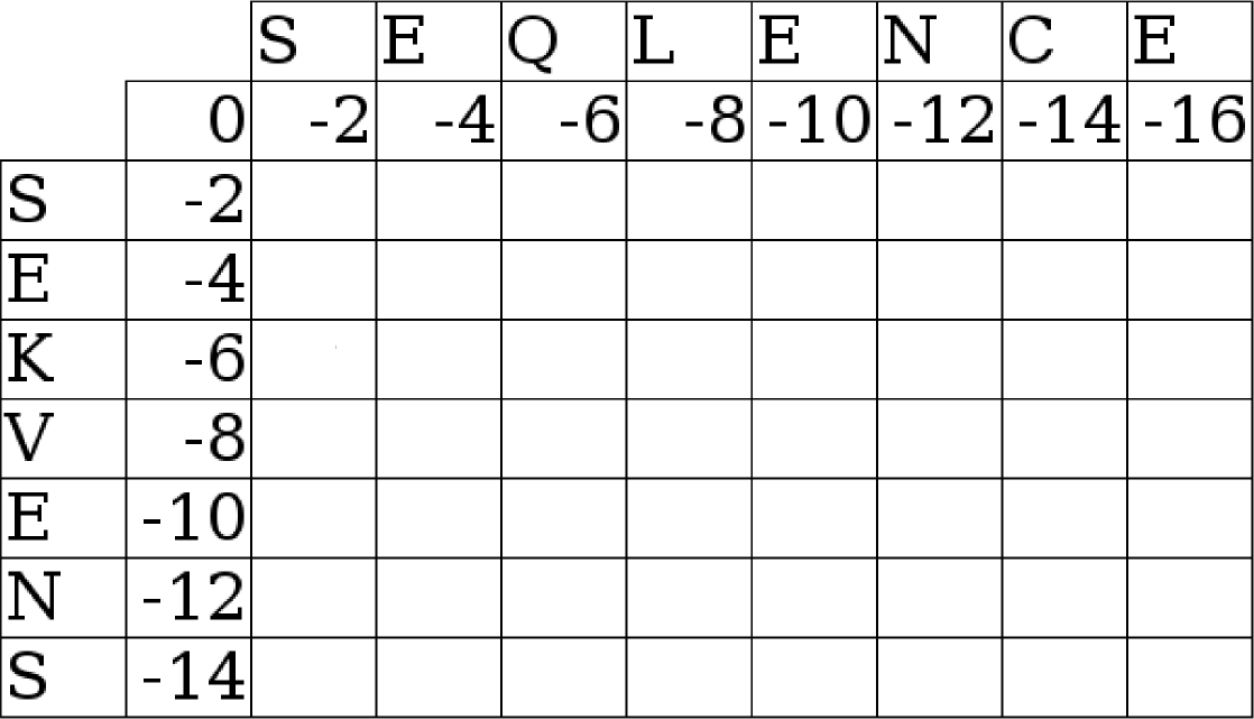
\includegraphics[width=0.4\textwidth]{fig/dynprog_example1.png} & 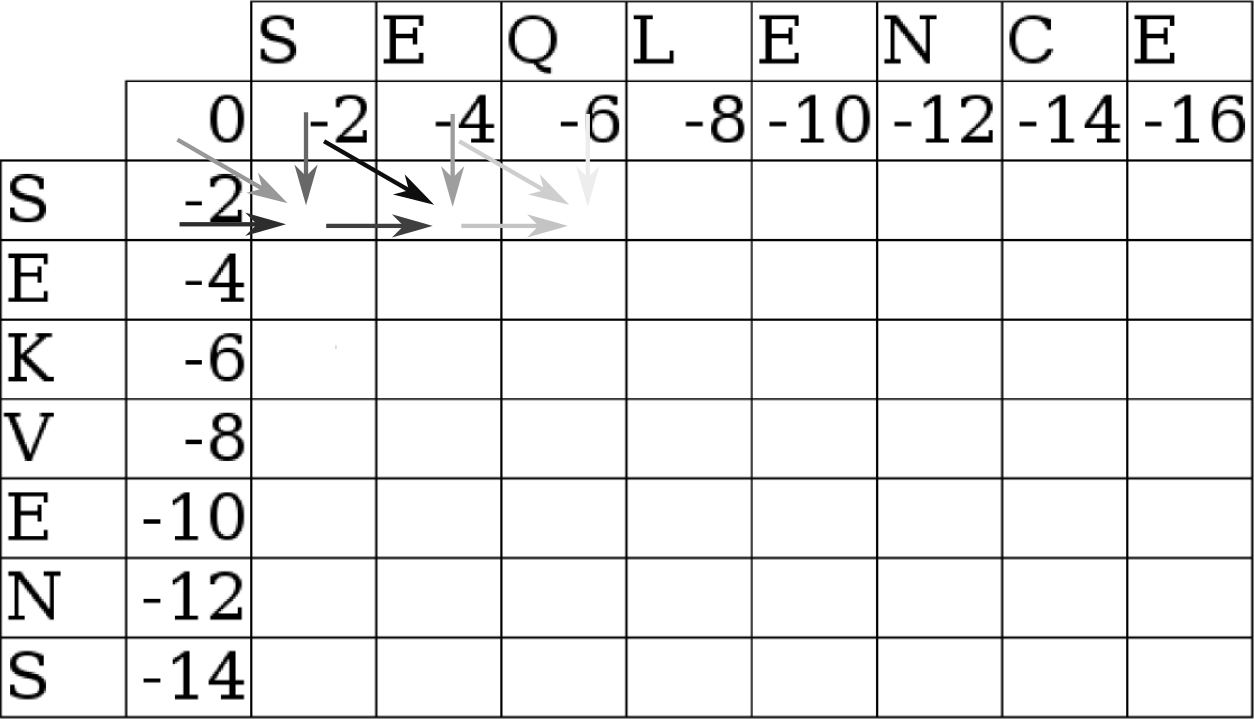
\includegraphics[width=0.4\textwidth]{fig/dynprog_example2.png}\\
 {\bf A} & {\bf B}\\
 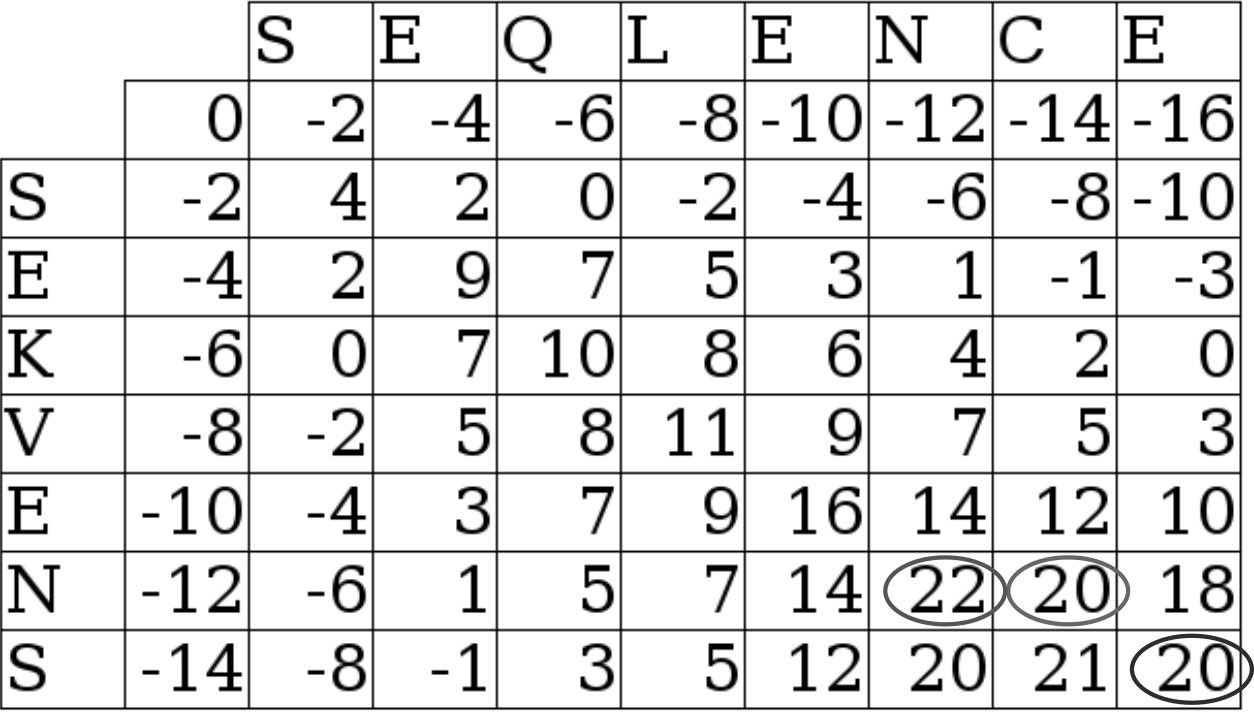
\includegraphics[width=0.4\textwidth]{fig/dynprog_example3.png} & 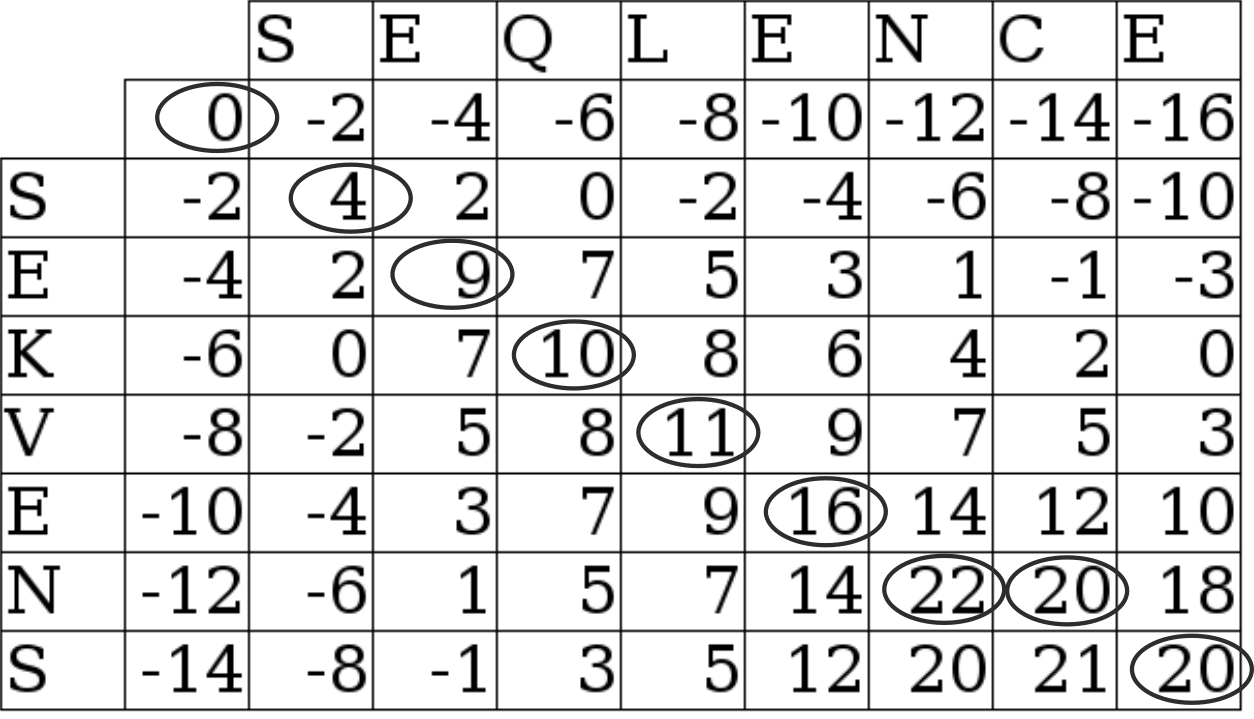
\includegraphics[width=0.4\textwidth]{fig/dynprog_example4.png}\\
 {\bf C} & {\bf D}\\
 \end{tabular}
 \caption{Dynamic programming algorithm for the sequences SEKVENS and SEQLENCE with BLOSUM62 and gap penalty: --2. A: Adding default gaps. B: Calculation of the matrix; match/gap/gap for each field. C: Matrix fully calculated, starting traceback. D: Calculations done. The final alignment is SEQLENCE vs SEKVEN-S.}
 \label{fig:dynprog_example}
\end{figure}

The algorithm for pairwise local alignments is very similar to the one for global alignment\cite{smith_identification_1981}. The basic algorithm is the same, but the scoring step has another condition added (equation \ref{eq:sw_field}) and the traceback starts in the field with the highest score and finished when it reaches a field with 0.

\begin{equation}
     F(i,j) = \max 
    \begin{cases}
      F(i-1,j-1) + s(x_i, y_j)\\
      F(i-1,j) - d\\
       F(i,j-1) - d\\
       0
    \end{cases}
    \label{eq:sw_field}
\end{equation}

The process of aligning two sequences, called pairwise alignment, is generally considered solved by dynamic programming\cite{needleman_general_1970, smith_identification_1981}, resulting in the optimal alignment based on the given parameters, i.e. scoring matrix and gap score. 

There are other algorithms for performing pairwise alignments, e.g. FOGSAA\cite{chakraborty_fogsaa:_2013}, which are much faster than the original dynamic programming approaches, but are not guaranteed to always provide the optimal alignment. The original methods thus still have a place to fill.


\subsubsection{Multiple Sequence Alignments}
\label{sec:msa}

It is often of interest to align more than two sequences in order to obtain more information about the sequence properties, as well as to study the similarities within e.g. a protein family.

Sadly, dynamic programming cannot be efficiently extended to aligning more than two sequences, as the number of required computations increases exponentially with the number of sequences. Thus, a number of alternative approaches have been developed to make MSAs, sacrificing the promise of providing optimal alignments for speed. Many of the current methods start by comparing the sequences pairwise, generating a guide tree showing which sequence have the highest level of similarity. The alignment is then generated by adding the sequences to the alignment in the order given by the guide tree, a process called progressive alignment. The accuracy of the alignment can be improved by e.g. iterative realignment processes during the ``alignment'' merging. Modern methods often include approaches as well, including e.g. fast Fourier transformations and HMMs.

There are multiple MSA methods available, and the choice of method is often a balance between accuracy and speed. The accuracy is also dependent on the properties of the sequences, e.g. the amount of insertions, different methods providing better alignment for different types of sequences. The accuracy of the methods can be evaluated by e.g. manually curated alignments such as BAliBASE\cite{thompson_balibase_2005}, but simulated sequences are also common in order to get larger sequence sets with controlled properties. Based on a benchmarking of multiple modern MSA methods\cite{pervez_evaluating_2014}, the most accurate methods include ProbCons\cite{do_probcons:_2005} and the L-INS-i approach of MAFFT\cite{katoh_mafft:_2002,katoh_mafft_2013}, while e.g. Kalign\cite{lassmann_kalign--accurate_2005,lassmann_kalign2:_2009} and the FFT-NS-2 approach of MAFFT are very fast (but less accurate). Depending on the types of sequences, other methods such as MulAlin\cite{corpet_multiple_1988} and SATe\cite{liu_rapid_2009,liu_sate-ii:_2012} are also good choices. Clustal Omega\cite{sievers_fast_2011} is often a good trade-off between speed and accuracy.


\subsection{Finding Homologs in Sequence Databases}
\label{sec:method_find_homologs}

When working with proteins, a very common objective is to find homologs to the current protein in the major sequence databases, e.g. UniProt and NCBI. There have been multiple methods developed for this purpose, both general and specialised ones. 


\subsubsection{BLAST}
\label{sec:method_blast}

The de facto standard for performing sequence searches in databases is the Basic Local Alignment Search Tool (BLAST) \nomenclature{BLAST}{Basic Local Alignment Search Tool} \cite{altschul_gapped_1997, camacho_blast+:_2009} suite of programs, covering searches for both nucleotide (blastn) and protein (blastp) sequences, and even automatic translation of nucleotide sequences to protein sequences (blastx) and vice versa (tblastn).

The original BLAST algorithm was published in 1990\cite{altschul_basic_1990} and is based on the concept of words (short regions with similar, not necessarily identical, residues), in contrast to the main sequence search software that existed at the time, FASTA\cite{lipman_rapid_1985}, which was searching for kmers of identical residues. This allowed BLAST to identify more distant homologs then was previously possible.

The algorithm starts by identifying words that would score above a certain threshold (using e.g. BLOSUM62), followed by matching of the words towards a sequence from a database. Regions with multiple words are extended into local alignments using dynamic programming. The local alignments with scores above a certain threshold are then reported as hits. The quality of a BLAST hit is commonly presented as an E value representing the probability of discovering a sequence with the current score in a database of the current size, but for e.g. short hits, other evaluation methodologies are commonly used, e.g. the sequence identity. 

\begin{figure}[htbp]
 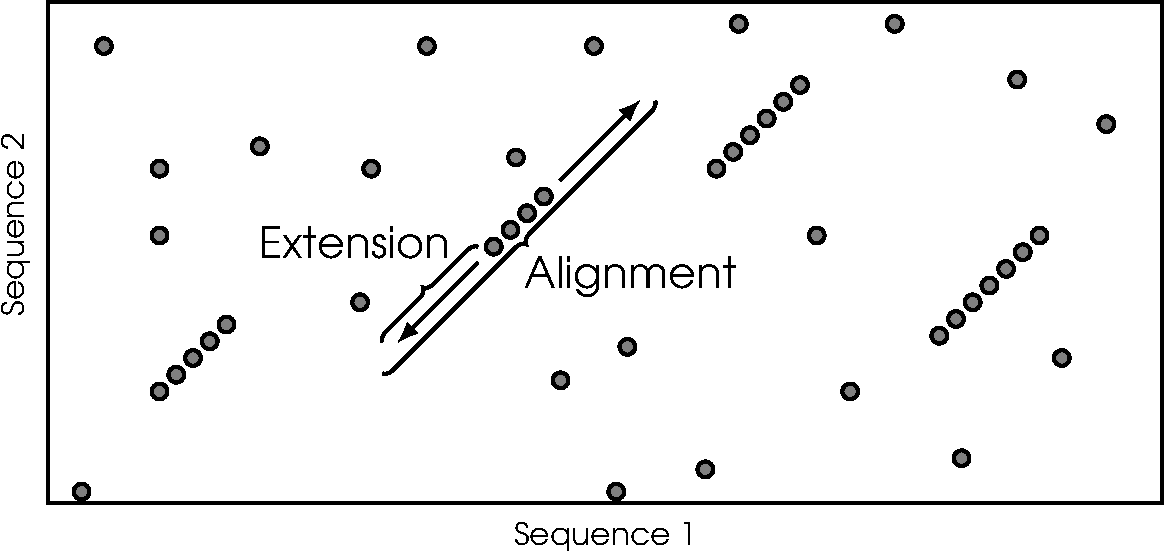
\includegraphics[width=0.9\textwidth]{fig/blast_method.pdf}
 \caption{The BLAST algorithm. The sequences are matched against high-scoring words (gray), and regions with multiple words are used as seeds for a local alignment that is extended until a defined threshold. Local alignment above the score threshold are then reported as results. {\em Modified from image by Per Unneberg}}
 \label{fig:blast_procedure}
\end{figure}

The standard BLAST method performs well for close homologs, but lacks sensitivity in regard to distant homologs. For this purpose, an iterative version of BLAST was developed; position-specific iterative BLAST (PSI-BLAST)\cite{altschul_gapped_1997}. \nomenclature{PSI-BLAST}{Position-specific iterated BLAST} PSI-BLAST starts by performing a normal BLAST search using e.g. BLOSUM62 as scoring matrix, but then the alignments of the results from the first search (iteration) are merged and a position-specific scoring matrix (PSSM) \nomenclature{PSSM}{Position-specific scoring matrix} is calculated, keeping the data for the positions in the original query sequence. Another iteration is then started, but the alignments are scored using the PSSM instead of the original scoring matrix. The search can then be iterated, generating a new PSSM with each iteration, until the search has converged (no new sequences are found).

Further specialised versions of BLAST have also been developed, including e.g. DELTA-BLAST\cite{boratyn_domain_2012}, which adds information from domain databases to the search to make it more accurate and sensitive for distant homologs.


\subsubsection{HMMER}
\label{sec:hmmer}

A protein or nucleotide sequence can be described as a hidden Markov model (HMM).  \nomenclature{HMM}{Hidden Markov model} By adding states corresponding to the residues/nucleotides at each position, as well as for insertions and deletions, the HMM can then be used to evaluate the similarity of other sequences to the original sequence. If an MSA containing sequences from e.g. the same proteins family is used to generate the HMM, the HMM can thus be used to evaluate whether other sequences belong to the same family. A common program for this purpose is HMMER\cite{eddy_accelerated_2011}, which also has a special module called JACKHMMER which can be used for the same purpose as BLAST, i.e. to find similar sequences in sequence databases.

Using the HMMs generated by HMMER, it is possible to create automated classifiers for protein families, as have been done for e.g. domains in the database Pfam\cite{finn_pfam:_2014}. 

Using HMMs is also useful when the goal is to separate e.g. a protein family into its members. E values and similar scores evaluate the probability of a sequence being a homolog, which should be true for all the members within the family. If an HMM is defined for each of the possible member proteins, then the HMM having the highest probability for a match should be the correct member, as was done for the six classes of ADH in paper \ref{paper:mammalian_adhs}.


\subsection{Evolutionary Relationships}
\label{sec:evolutionary_rel}

It is often of interest to study the evolutionary relationships between proteins. In its traditional form, phylogeny is used to study the evolutionary relationship between species, but phylogenetic methods, e.g. PhyML\cite{guindon_new_2010}, can also be used to study the relationships between protein families.

Phylogenetic trees visualise the evolutionary relationships between species or proteins. All species or sequences, depending on what is compared, are visualised as nodes in a tree graph, while the edges show the relations. There are multiple different types of trees, but many scale the branches according to the ``evolutionary distance'' between the species or sequences that are compared.


\subsubsection{Evolutionary Pressure}
\label{sec:evolutionary_p}

Evolution is an ongoing process, and all nucleotide and protein sequences will change over time to a varying degree. As the function of a gene is most commonly performed by the encoded protein, the preservation of the amino acid sequence is of importance. If the sequence changes in a way that makes the protein less efficient for its purpose, the organism will have an evolutionary disadvantage, and thus there is an evolutionary pressure to maintain the same sequence. The mutations occur at the DNA level, and as many amino acid residues are encoded by multiple different codons, a change may either be non-synonymous or synonymous, i.e. the mutation will or will not change the encoded residue.

If the function of a protein has become less important due to e.g. changes in the environment surrounding the organism, the evolutionary pressure will decrease, as the loss of efficiency for the protein will not cause the same evolutionary disadvantage, and thus more non-synonymous mutations are accepted. As the mutations occur over time, a gene that recently lost its importance may still have the characteristics of a gene. One way of evaluating the level of evolutionary pressure is to compare nucleotide sequences from different species and simulate how they were changing, and then calculating the quotient $\frac{non-synonymous}{synonymous}$, or in short $\frac{dN}{dS}$. If the result is greater than 1, i.e. there are more non-synonymous than synonymous mutations, it strongly implies that the gene is ``disappearing'' from the genome. As a reference,  the mammalian members of the highly conserved histone H1 has a ratio of 0.055, while the highly variable interleukin-2 has a ratio of 0.556\refpaper{paper:adh5_2016}. There are many methods for performing such calculations, a common one being PAML\cite{yang_paml_2007}.


\subsection{Conservation}
\label{sec:conservation}

Connected to the concept of evolution is the concept of conservation: what parts of the sequence are conserved by the evolutionary pressure?

The common approach to evaluate the conservation is to collect sequences from multiple species, perform a multiple sequence alignment and evaluate the results. The important residues in a protein are often conserved even in distantly related species, as well as within a protein family.

How distantly related the sequences that are included in the alignment should be is based on what property is of interest. In the case of MDRs, the properties of the binding pocket for NAD(P)H is expected to be similar between the species, and comparing the conserved residues in proteins binding NAD(H) with the ones in proteins binding NADP(H), it is possible to identify residues are responsible for the selection of coenzyme.

The same approach can theoretically be used to identify the active site in an enzyme, but the choice of included sequences is then very important, as evidenced by the results in Paper \ref{paper:mammalian_adhs}. If the sequences do not share the same type of active site, the obtained results will be inaccurate.

Finally, the conserved residues can be mapped to structures to evaluate their localisation; are they part of the active site, important for protein-protein interaction, or maybe have some other functions?


\section{Structure}
\label{sec:methods_structure}

While the sequence of a protein is the raw results of the expression of a gene, the way it folds is crucial for its function. Thus, the structure of a protein is more conserved than its sequence. It also means that there is a strong incentive to determine as many protein structures as possible.

The common methodology for determining structures are X-ray crystallography, NMR, and electron microscopy, X-ray crystallography being the most common with nearly 90\% of the structures in the PDB. The number of determined structures is growing, and as of March 2017, there are more than 125,000 structures deposited to the PDB\cite{noauthor_rcsb_nodate}.


\subsection{Predicting Protein Structure}
\label{sec:struc_pred}

The structure has been determined for a large number of proteins, but the structures of a vastly greater number of proteins remain to be determined, and the number of proteins without known structure increases much faster than the number of proteins with known structures.

One way of bypassing this problem is to use computational methods to predict the structure based on its sequence. Sadly, the folding of a protein cannot be solved by a simple and straight-forward approach. The protein folding (Levinthal's) paradox\cite{levinthal_how_1969} states that the number of possible conformations available to a given protein is extremely large, and a brute-force method exploring all conformations of even a small 100-residue protein would take longer to finish than the universe has existed. Thus, an algorithm attempting to predict a protein structure would need to use shortcuts.

There are a multitude of methods developed for ab initio structure predictions with energy-based and fragment-based approaches, using physical principles to predict a probable structure, often requiring considerable computational resources.

Another ab initio approach that has been gaining a lot of traction is to use evolutionary covariation for the predictions, the idea being that residues that mutate together should be located near each other in the protein structure. This approach has been quite successful and there are multiple methods developed, e.g. EVfold\cite{marks_protein_2011}. There are also methods that combine multiple different approaches, such as PconsE, which combine the coevolutionary analysis of PconsC\cite{skwark_pconsc:_2013} with the ab initio-approach used in the Rosetta suit of programs\cite{simons_assembly_1997}.

There is also another type of protein structure prediction method that attempts to use proteins with known structure as templates for the prediction, called homology modelling (or sometimes template-based modelling).

In its simplest form, a homology modelling method would use the structure of a homolog to the protein of interest and copy the backbone from the parts that have high levels of similarity between the structures. The method would then connect the copied parts by generating the missing regions using e.g. ab initio methods, but with the template structure as a starting point. The generated structure model would then be refined, often using e.g. energy minimisation.

\begin{figure}[htbp]
 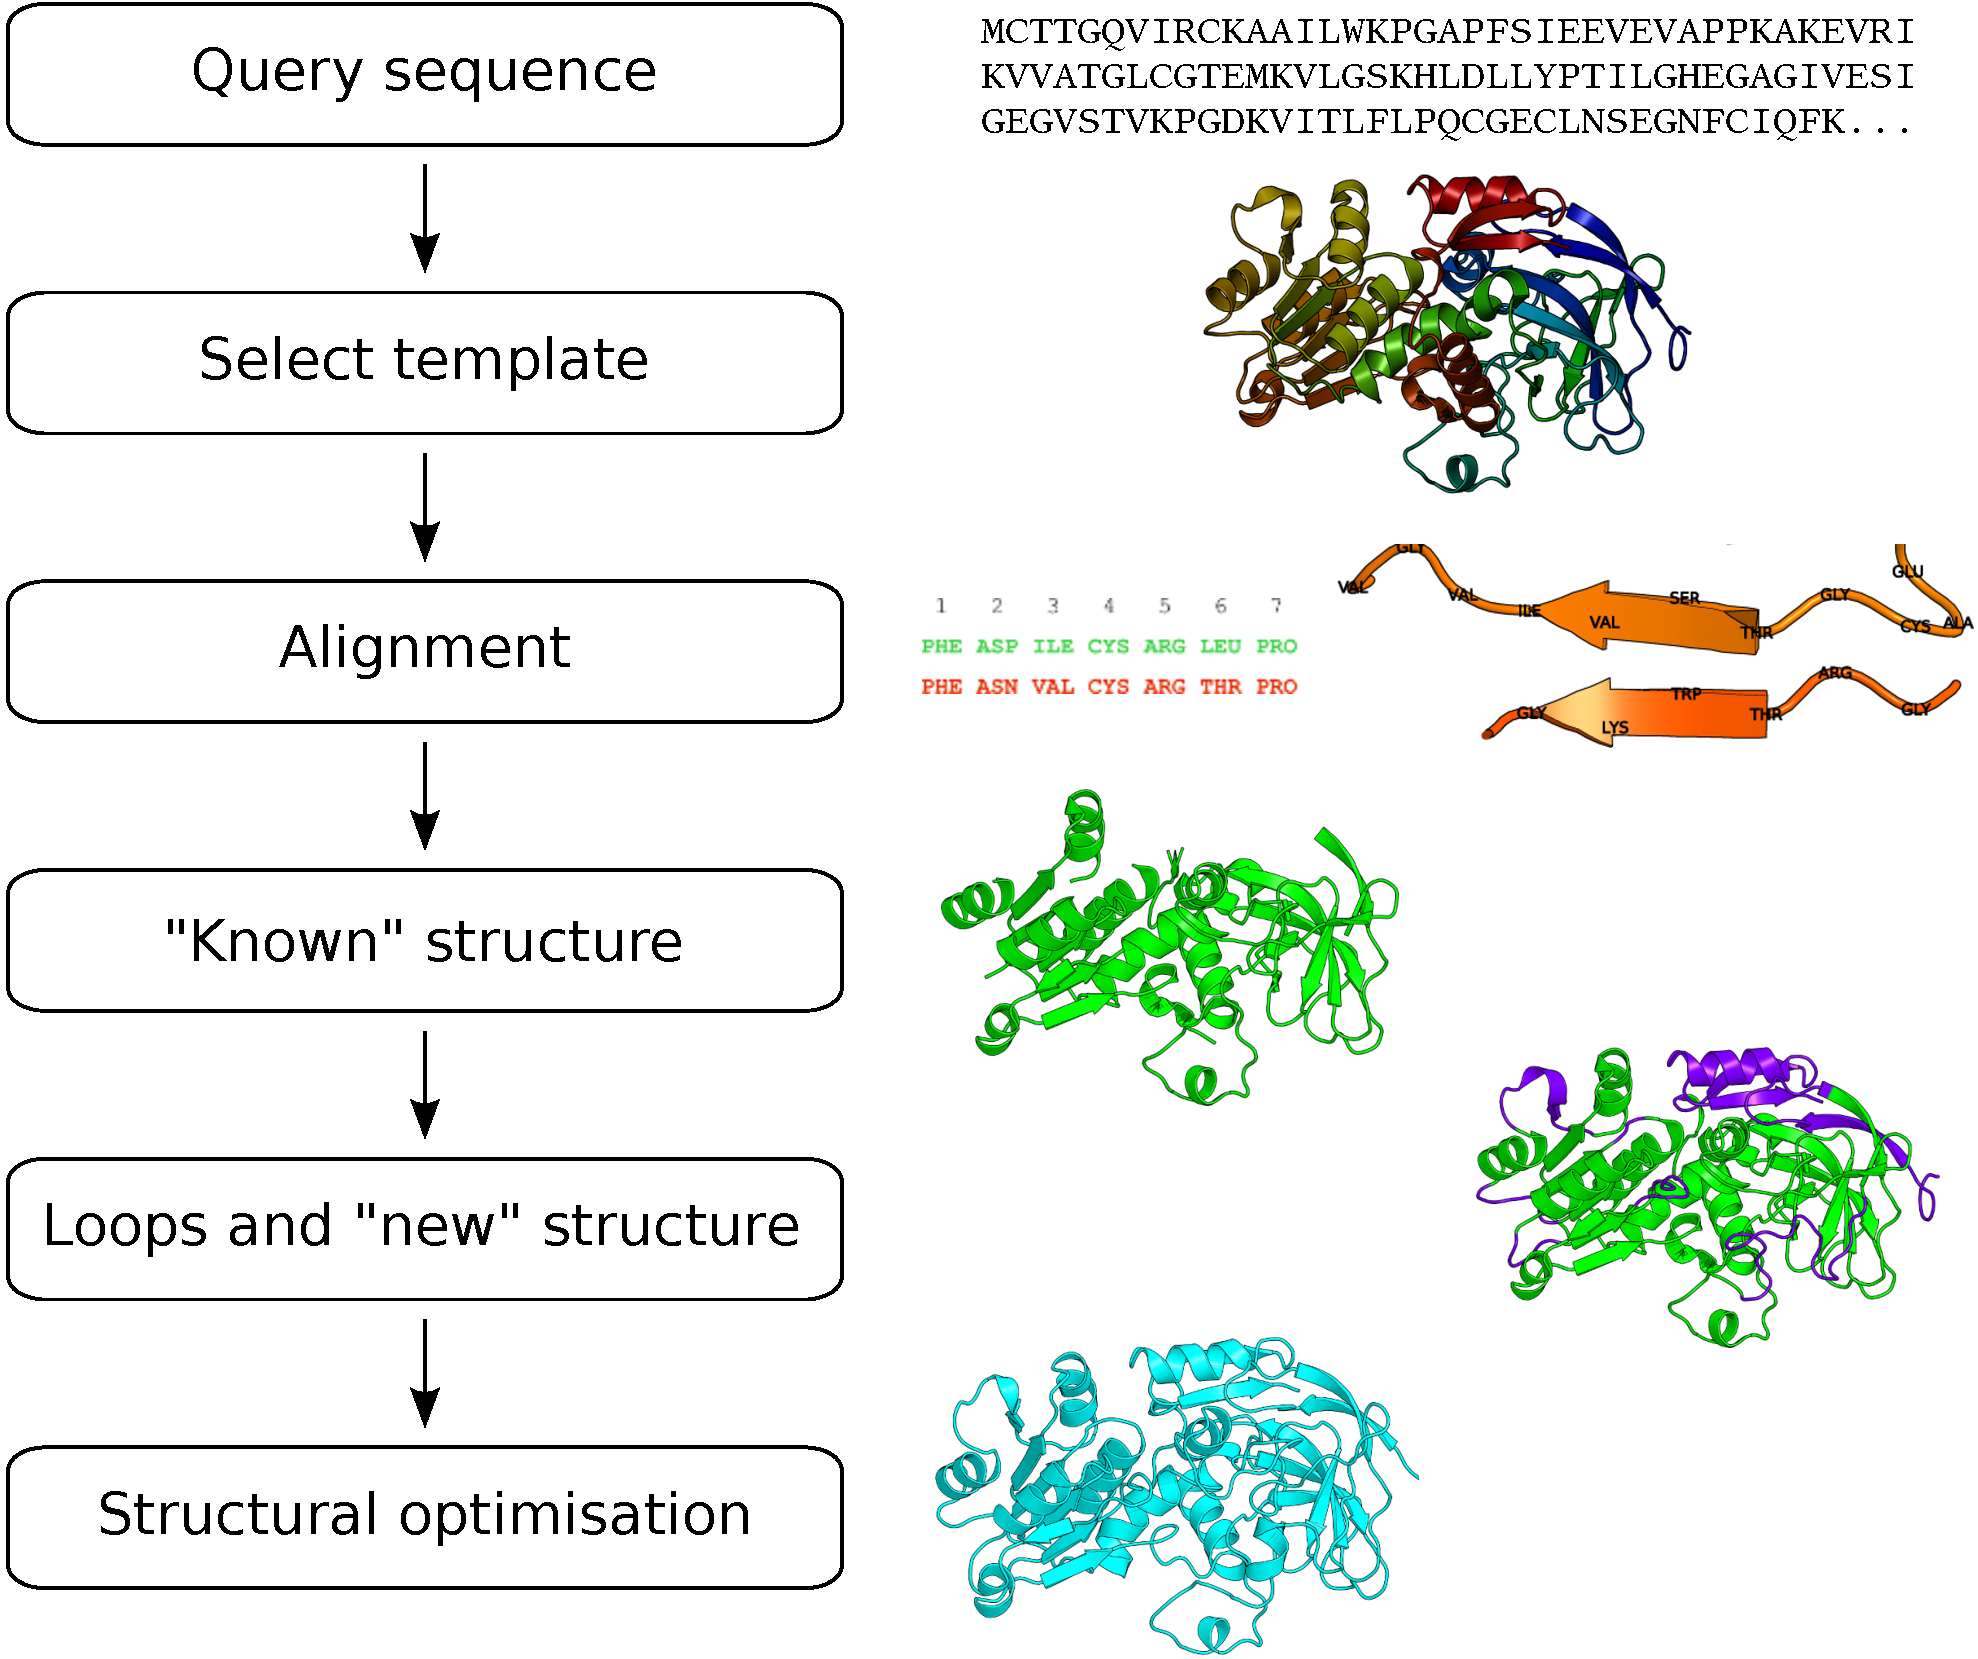
\includegraphics[width=0.8\textwidth]{fig/hom_mod.pdf}
 \caption{Schematic representation of a general homology modelling method}
 \label{fig:hom_mod_procedure}
\end{figure}

As homology modelling uses homologs as templates, the methodology is heavily dependent on the availability of close homologs with known structures. There are also variations of the template identification approach that matches the sequence to known structures, evaluating whether the sequence could form the structure in question, rather than evaluating whether they are homologous.

There are a large amount of homology methods available, including e.g. MODELLER\cite{sali_comparative_1993}, SWISS-MODEL\cite{arnold_swiss-model_2006}, and I-TASSER\cite{roy_i-tasser:_2010}. More methods are constantly being developed, improved by new algorithms, not to mention the increasing amount of possible template structures in the PDB.

In the case of MDRs, the standard homology modelling methods often provide very good models in regard to the backbone of the protein. However, as many MDRs also bind cofactors, e.g NAD(H)/NADP(H) and Zn$^{2+}$ ions, which are difficult to add after the model refinement steps, the models generated by the standard methods are often suboptimal for MDR enzymes.

In the projects forming this thesis, the most common approach was to use a modified homology modelling approach from the ICM software. First a protein structure model was created using the standard ICM method\cite{abagyan_homology_1997}, whereafter the coenzyme(s) were added before refinement, during which all sidechains were forced into positions that allowed the coenzyme to stay in place before constraints were gradually relaxed and the protein structure model was allowed to find its local energy minimum.


\subsection{Studying the Dynamics of a Protein}
\label{sec:prot_dyn}

When a protein is successfully crystallised, the crystal contains a large amount of individual copies of the protein in the same (or similar) conformations. When the crystal is scanned with X-rays, the refraction patterns can be used to determine the structure. If the individual copies of the protein are all in the exactly same conformation, the refraction pattern will be stronger and the structure can be inferred. If the conformation of a part of the protein varies between the individual protein copies, there will be multiple refraction patterns, and all of them will be weaker, making it more difficult to give an accurate representation of that part of the structure.

As an effect of this, all crystal structures are static, i.e. showing only one conformation of the proteins. As proteins are dynamic, constantly varying the structure to allow e.g. the binding of substrates, a crystal structure cannot represent the full array of different conformations a protein can have. The dynamics of a protein can be studied using NMR, though it mainly works on small proteins. Instead, the dynamics of a protein can be simulated in silico using molecular mechanics.

The two main approaches in molecular mechanics for proteins are Monte Carlo and molecular dynamics (MD) \nomenclature{MD}{Molecular dynamics} methods. The Monte Carlo methods performs random changes to the system and evaluates their results, generating an ensemble of configurations, giving information about different states for the protein\cite{paquet_molecular_2015}. The MD methods instead simulate the the movement of the atoms over short timesteps.

The general properties and equations describing the properties and interactions between atoms are often referred to as the force field. Any calculations on a molecular system would preferably use quantum mechanics, but as those calculations are very computationally intensive, they are infeasible for large systems such as proteins, especially when the behaviour over larger time scales are simulated. Instead the methods uses approximations that are considered to be accurate enough, but may lack in their exact representation of e.g. hydrogens. Thus, molecular dynamics uses Newtonian (classical) mechanics and approximate representations of e.g. van der Waal interactions to calculate how the system behaves over time.

As proteins are commonly not performing their functions in a vacuum, it is a good idea to simulate e.g. water around the protein molecule, either explicitly (with added water molecules) or implicitly (using general equations to describe the interactions of the protein with a general water environment). The addition of water molecules adds a lot of new atoms to the calculations, increasing the amount of required calculations when compared to implicit water, but may generate more accurate results by e.g. explicitly simulating water molecules that are interacting with the protein.

GROMACS\cite{abraham_gromacs:_2015}  is an open source implementation of a molecular mechanics system, performing energy minimisation (finding local energy minima) and molecular dynamics, that was originally developed at the Groningen University in 1991. It is able to use different force fields and is highly optimised for speed by using optimised CPU instructions as well as supporting heterogenous systems (CPU + GPU) for a further performance boost\cite{abraham_gromacs:_2015}.


\chapter{Present Investigations}
\label{sec:projects}

\section{Aim}
\label{sec:aim}
\begin{itemize}
 \item To identify mammalian alcohol dehydrogenases in the databases and to investigate that their annotations match their real classification (class I--VI), including analysis of the identified members and their relationships (paper \ref{paper:mammalian_adhs}; section \ref{sec:mammalian_adhs}).
 
 \item To study ADH5, first attempting to isolate and characterise it, followed by computational analysis of the structure of human ADH5 as well as the sequences of ADH5 from other mammals (paper \ref{paper:adh5_2013} and \ref{paper:adh5_2016}; section \ref{sec:adh5}).
 
 \item To define important residues in the binding pockets of MDRs, focusing on nine different MDRs that are present in humans and for which only little is known (paper \ref{paper:mdrs}; section \ref{sec:mdr_pocket}).
 
\end{itemize}


\section{The Mammalian Alcohol Dehydrogenases}
\label{sec:mammalian_adhs}

With the constant inflow of new sequences to the UniProt and NCBI sequence databases, there is also a constant inflow of new mammalian ADH sequences. Most of the sequences are correctly annotated, but there are also multiple ones that are not annotated at all (``uncharacterized protein''), or in some cases annotated as belonging to the incorrect class.

The aim of this project (paper \ref{paper:mammalian_adhs}) was to summarise the mammalian ADHs currently available in the aforementioned sequence databases.

At the core of the project was the development of a pipeline that could be used to identify ADH members, confirm that they were correctly classified, and then add them to a local SQLite 3 database (\url{www.sqlite.org}). A general visualisation of the pipeline is available in Figure \ref{fig:adh_pipeline}, showing the use of BLAST \cite{altschul_gapped_1997, camacho_blast+:_2009} to identify sequences and HMMER \cite{eddy_accelerated_2011} to confirm their classifications by matching the sequences against class-specific HMMs.

\begin{figure}[htbp]
 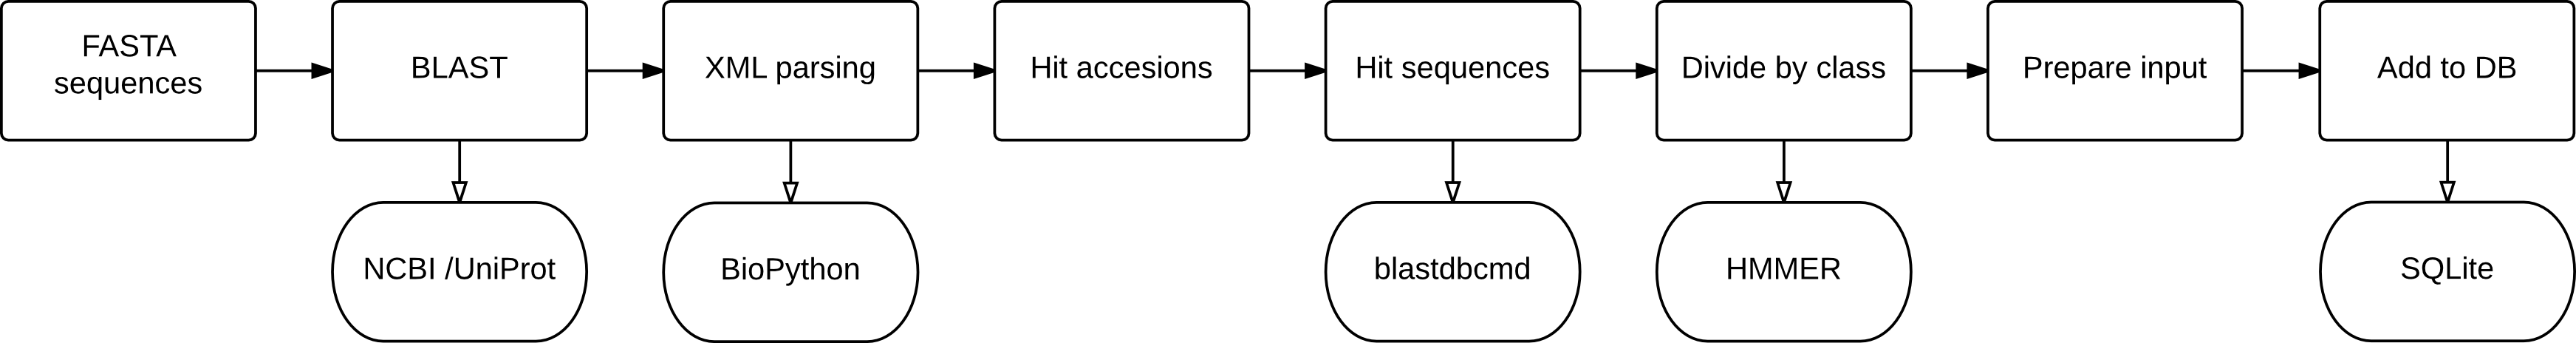
\includegraphics[width=\textwidth]{fig/adh_pipeline.png}
 \caption{Visualisation of the pipeline used to identify and classify alcohol dehydrogenases available in the major sequence databases.}
 \label{fig:adh_pipeline}
\end{figure}

As the pipeline was designed to automate the whole process, the pipeline could be reused for later updates. However, the design turned out to be suboptimal for continuous updates, as it did not include any checks to confirm that sequences that had already been added were still present in the databases. The original analysis (performed during summer 2014) identified a total of 584 sequences belonging to 85 different mammalian species. A new run, performed in March 2017, identified 941 sequences from 145 mammalian species. Thus, the number of known mammalian ADH sequences keep increasing along with the number of species with at least one known member.

Both the original and new data show that the databases should be updated with a new class, as the phylogenetic tree clearly shows six classes, rather than the five that are usually noted in the literature (Figure \ref{fig:adh_tree}). Many of the members of class VI ADH are currently misclassified as class V or ``class I-like''.

\begin{figure}
 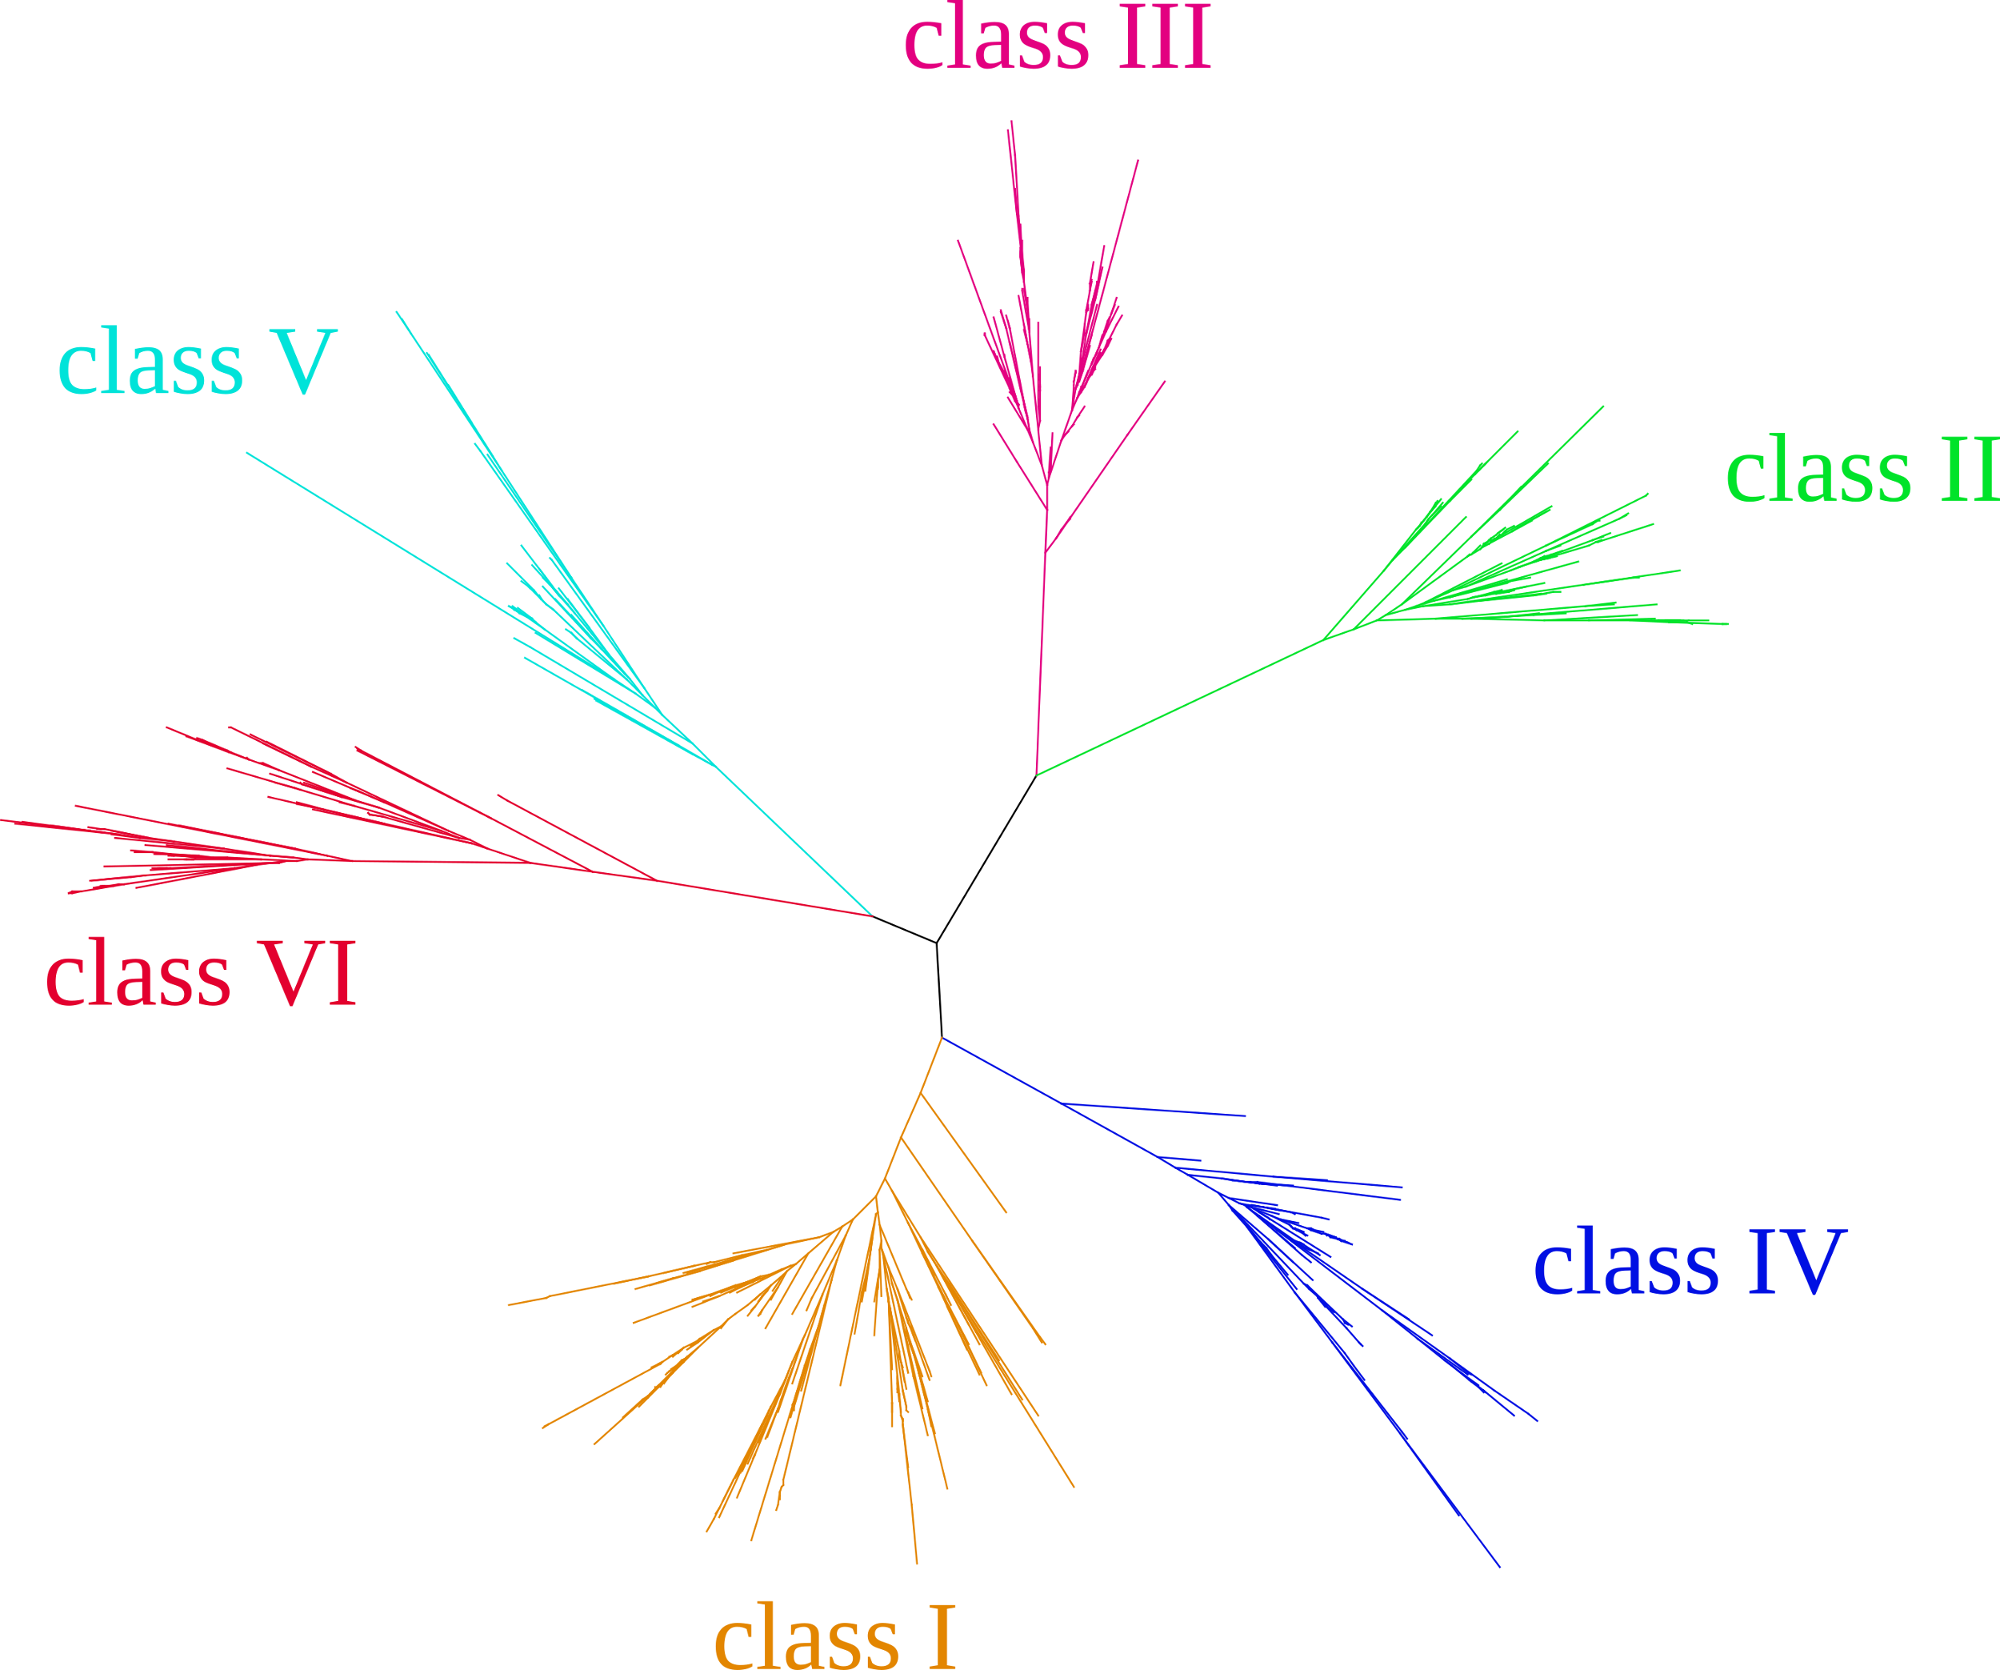
\includegraphics[width=0.8\textwidth]{fig/mammalian_adh_tree.png}
 \caption{Phylogenetic tree covering the known mammalian ADH se	quences as of March 2017.}
 \label{fig:adh_tree}
\end{figure}

The discovered sequences allowed further mapping of the mammalian ADHs. The number of ADHs in mammals varies between six in most non-primates to ten in vole, vole having four copies of ADH1 (ADH1:1--4), ADH2, ADH3, ADH4, ADH5, and two copies of ADH6 (ADH6A and ADH6B).

Three ADHs, namely ADH1, ADH2, and ADH6, have been duplicated in several species. Multiple copies of ADH1 are common in primates, but have also been observed in e.g. horses. Duplications of ADH2 have only been observed in hare animals, while ADH6 duplications have been observed in rodents.

Finally, many genomes still lack multiple expected ADH genes. The horse genome still lacks ADH2, ADH4, and ADH5, though ADH2 has been observed in Przewalski's horse \href{https://www.ncbi.nlm.nih.gov/protein/664777432}{[NCBI: XP$\_$008508014.1]}. The genes may have become pseudogenes, but their presence in related species imply that even genomes that are considered fully sequenced can still be improved.


\section{Class V Alcohol Dehydrogenase}
\label{sec:adh5}

The class V alcohol dehydrogenase (ADH5), often called ADH6 in the sequence databases (Table \ref{table:adh_nomenclature}), is a class of mammalian alcohol dehydrogenase with an as of yet unknown function. It was first identified using cross-hybridization with ADH1B cDNA probes in 1991\cite{yasunami_human_1991}. The same protein was also identified as cDNA in deer mouse in 1993\cite{zheng_molecular_1993}. The human protein was investigated in 1991\cite{chen_enzymatic_1991}, but as noted there, the data fits well with the ``class II stomach ADH'', which correspond to the at that time not yet discovered ADH4.

Originally, ADH5 was believed to lack the last exon present in other ADHs, the ninth, due to a splice variant, but transcripts containing the exon has since been discovered\cite{stromberg_human_2000}. In UniProt, the eight-exon variant is considered the main isoform with 368 amino acid residues, while the full version is annotated as isoform 2 with 375 amino acid residues.

The databases contain many misclassified ADH5 proteins, as most class VI ADHs are also annotated as ADH6, or even class V, sharing the annotation with most ADH5s in the sequence databases. As observed in section \ref{sec:mammalian_adhs}, while commonly located near the ADH5 branch in phylogenetic trees, the class VI ADHs clearly form a class of their own (Figure \ref{fig:adh_tree}).

Being the last non-characterised ADH isoform that is present in humans, it is of interest to investigate its function and characteristics. The work presented in paper \ref{paper:adh5_2013} and \ref{paper:adh5_2016} covers an investigation of this protein, starting with in vitro approaches (paper \ref{paper:adh5_2013}), and when the attempt to express and isolate the protein was unsuccessful, the focus shifted to computational methods (paper \ref{paper:adh5_2013} and \ref{paper:adh5_2016}).


\subsection{In Vitro}
\label{sec:adh5_vitro}

Performing Northern blot analysis of rat ADH5 showed a strong signal in kidney, corresponding to both splice variants. The shorter variant was also observed in liver, stomach, duodenum, and colon. This differs from the expression data found in the Human Protein Atlas\cite{uhlen_tissue-based_2015}, where the ADH6 entry notes high expression in liver, with kidney and the intestines having only low expression, similar to most other human ADHs. 

The rat and human ADH5 proteins were expressed in {\em E. coli} and COS cells, respectively. The expression in {\em E. coli} did not generate any soluble human ADH5, but a fusion protein with gluthatione-S-transferase (GST) \nomenclature{GST}{Gluthatione-S-transferase} could be expressed. However, this fusion protein did not show any activity with the traditional ADH substrates ethanol, octanol, benzyl alcohol, and hydroxymethylglutathione (HMGSH). \nomenclature{HMGSH}{Hydroxymethylglutathione} In the case of rat ADH5 in COS cells, the protein could be expressed as a fusion protein with green fluorescent protein (GFP), \nomenclature{GFP}{Green fluorescent protein} but again with no observed activity for ethanol, octanol, or HMGSH. A similar fusion protein construct with GFP-ADH3 did have the expected activity, implying that the GFP construct should be functional.

In short, the native proteins could not be isolated, and fusion protein constructs did not have any activity with the traditional ADH substrates.


\subsection{In Silico}
\label{sec:adh5_silico}

As the in vitro experiments did not yield any isolated ADH5 proteins, the focus was shifted to analysing the sequences and structure using computational methods.

Initially (paper \ref{paper:adh5_2013}), a model of rat ADH5 was generated using the MODELLER structure prediction method. The model was then analysed through a limited run of MD simulations using GROMACS, showing irregularities in the central $\beta$-sheets involved in the formation of dimers.

Continuing the analysis based on this observation, a model of human ADH5 was generated using a modified structure prediction method from the software ICM that was adapted to ADH analysis (paper \ref{paper:adh5_2016}). The irregularities around the dimer-interacting region were observed in the human model as well.

\begin{figure}[p]
 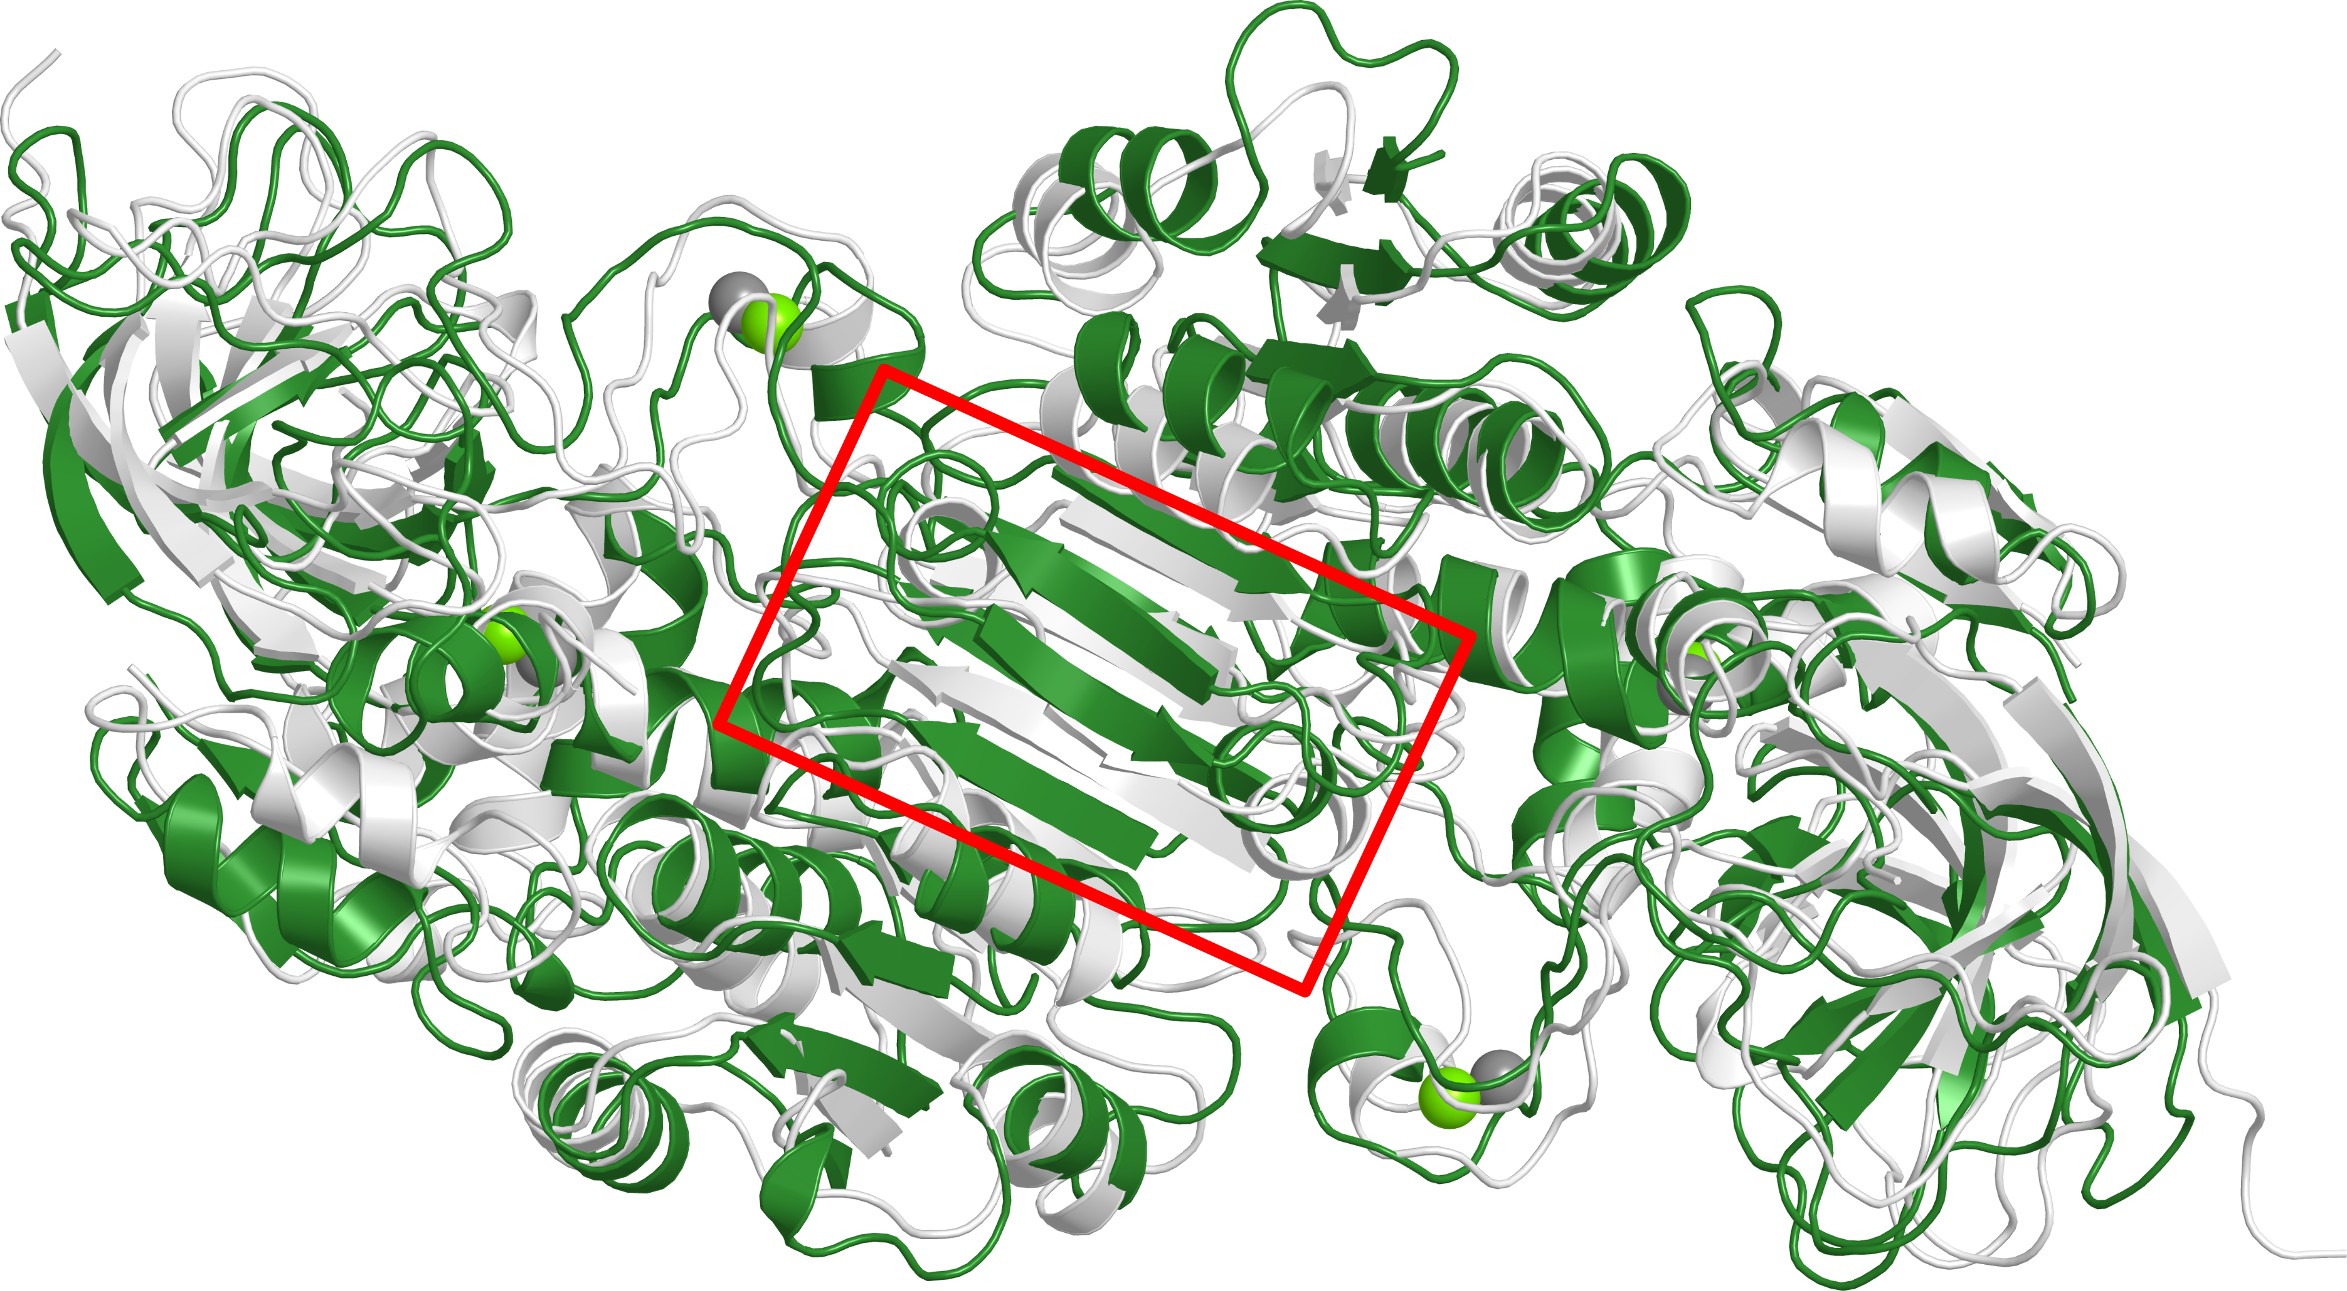
\includegraphics[width=0.9\textwidth]{fig/adh5_adh1_struct.png}
 \caption{Comparison between structural models of human ADH1C and ADH5 after 20 ns of MD simulations. Note the differences in the central region where the dimer interaction occurs. Source: paper \ref{paper:adh5_2016}}
 \label{fig:adh1c_5_model_comp}
\end{figure}

Along with the structural models, the sequences of multiple ADH5 proteins were also investigated. At the time of the initial investigation (paper \ref{paper:adh5_2013}), the number of ADH5 protein sequences in the databases was very limited, and there were only two mammals with at least one member in each of the six mammalian ADH classes. By the time of the continued investigation, the number had increased, with a total of 51 ADH5 sequences and ten species with at least one member per class.

\begin{figure}[p]
 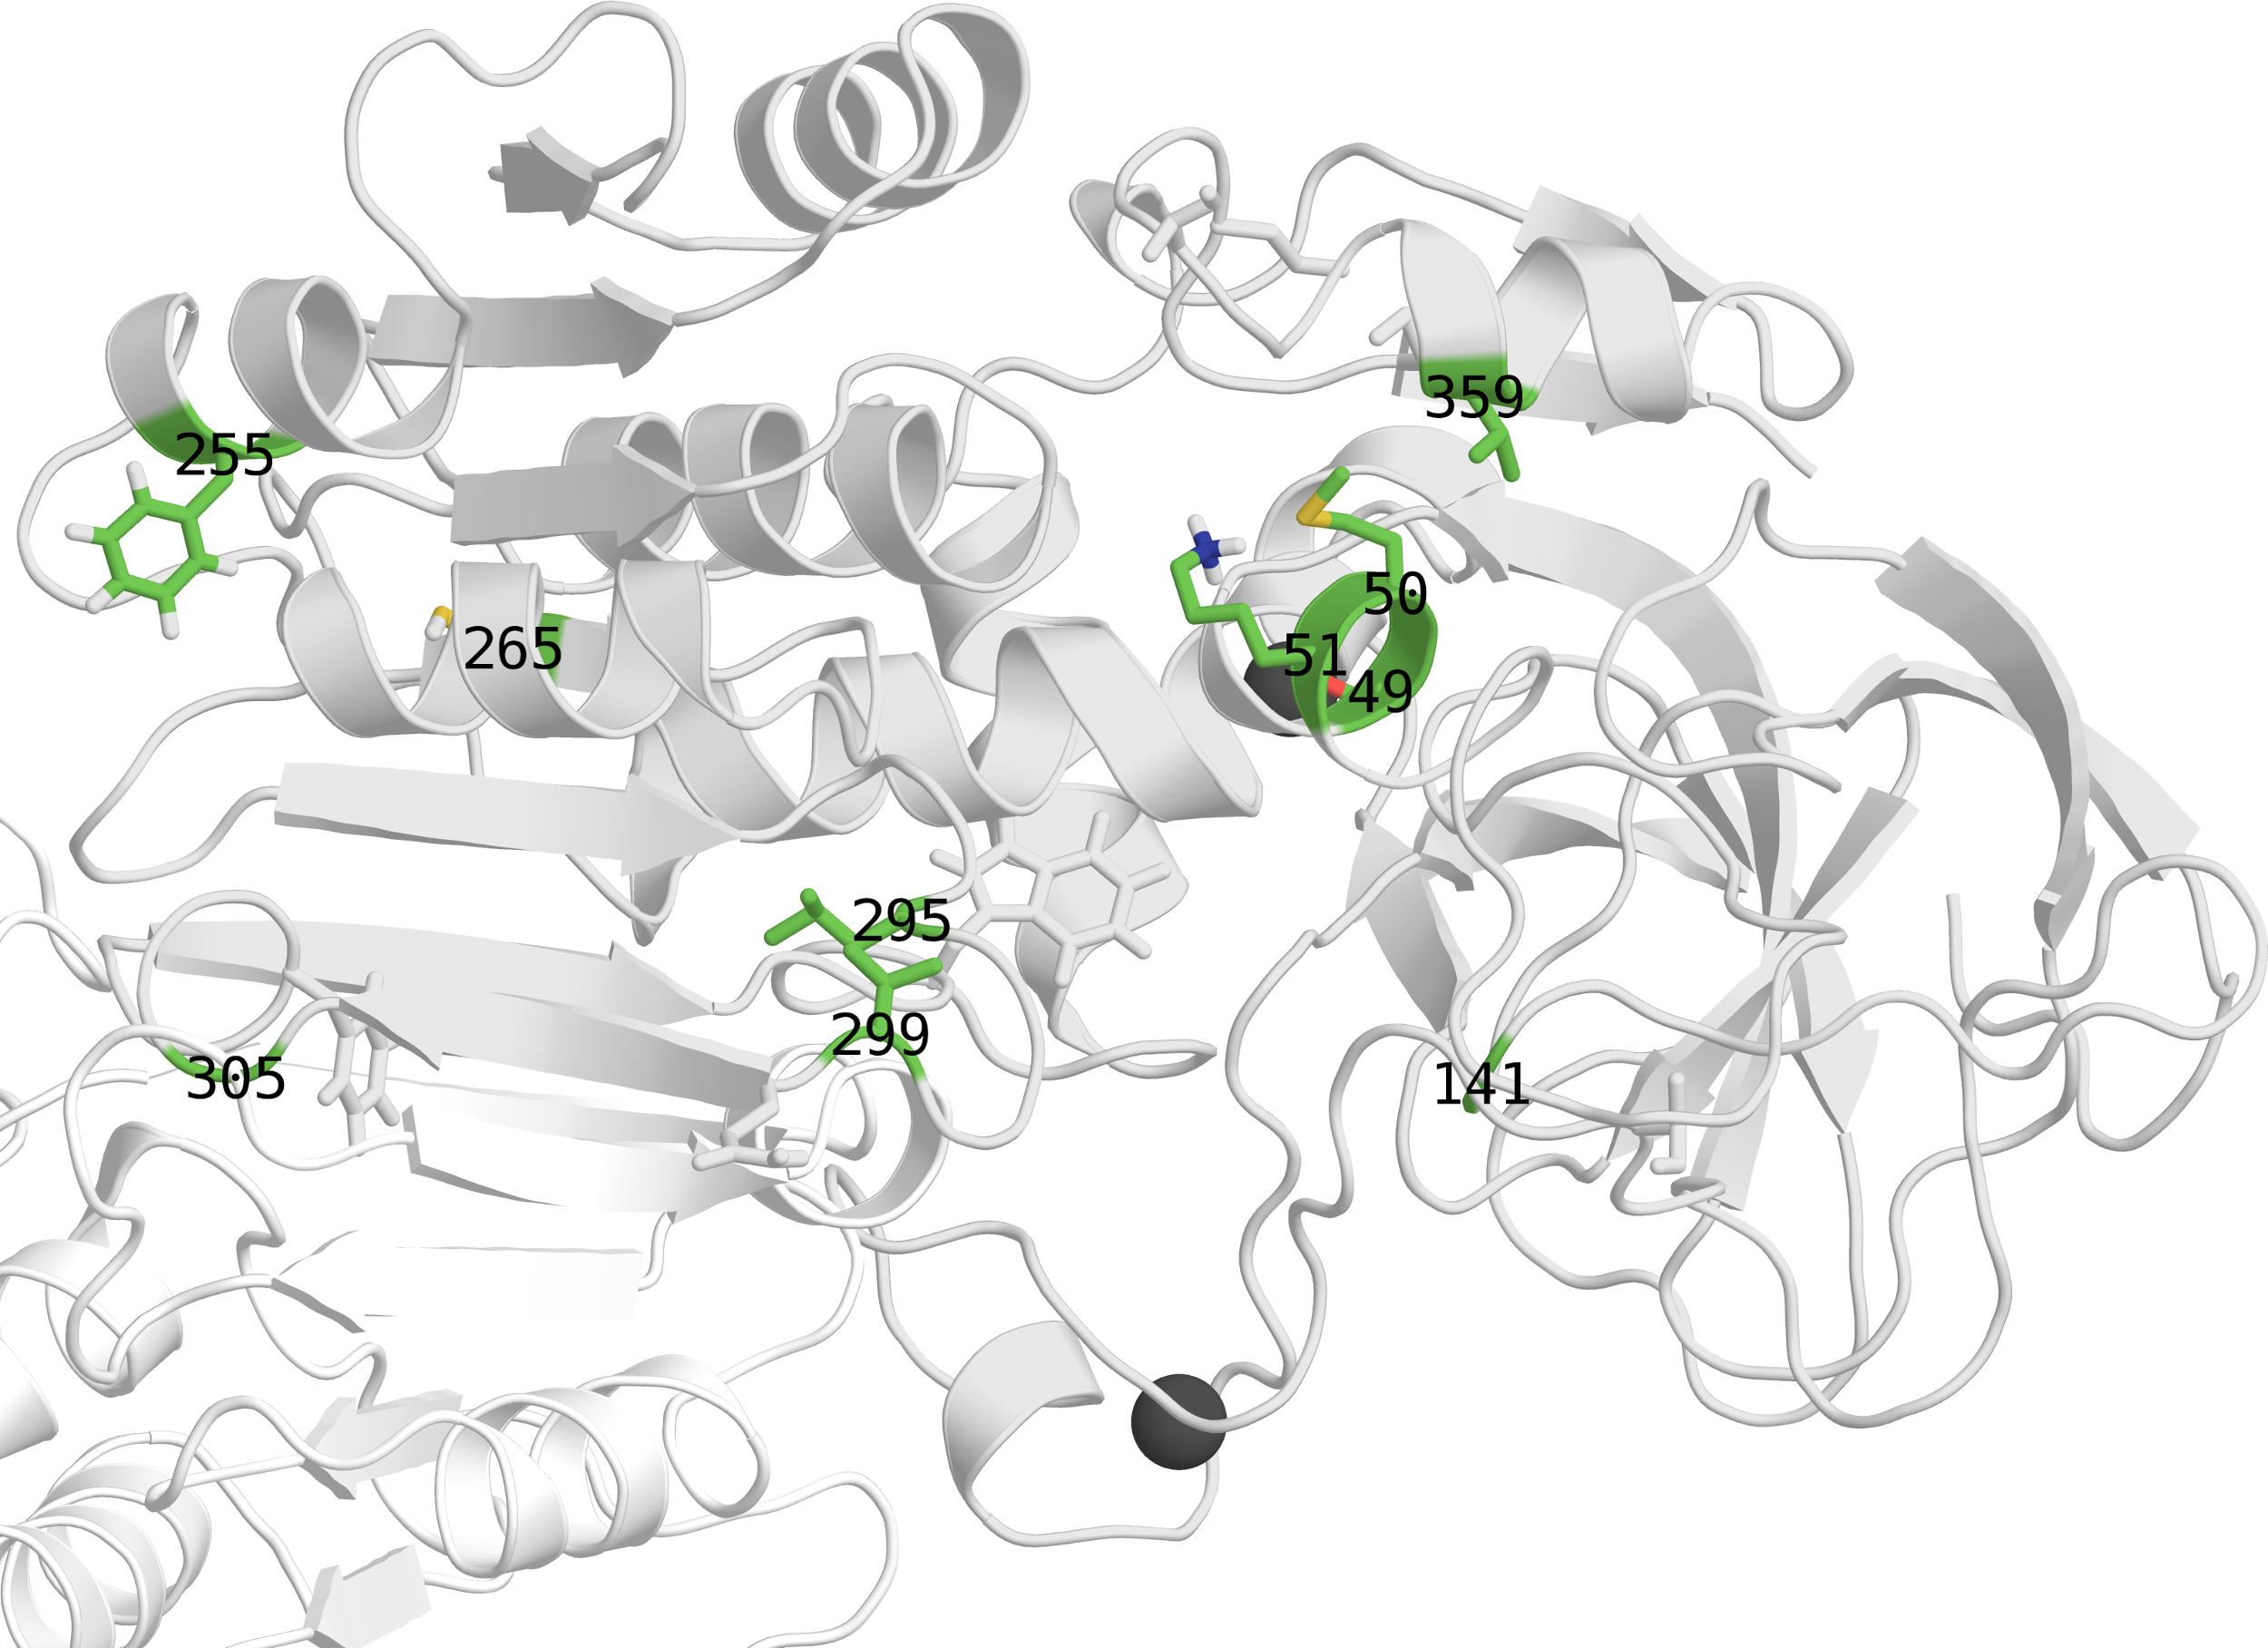
\includegraphics[width=0.9\textwidth]{fig/adh5_uniq_pos.png}
 \caption{Unique positions in ADH5 mapped to a structural model of the same protein. Source: paper \ref{paper:adh5_2016}}
 \label{fig:adh5_uniq_struct}
\end{figure}	

By analysing the conservation of the positions within each of the six classes, multiple amino acid residues were identified as unique for the ADH5 proteins, including some positions with near-perfect conservation in ADH1--4 and 6, but with a different residue in ADH5, e.g. Gly305, replacing a Pro in most other mammalian ADHs. In total, ten unique amino acid residues were identified, with Lys51 being the only one that was conserved among all the ADH5 proteins. Lys51 is located at the active site, with the other ADHs having His, Tyr, or Thr at this position\cite{hoog_mammalian_2001-1}.

Further, three residues, Leu295, Val299, and the aforementioned Gly305 were located in the dimer interaction region. Most classes of alcohol dehydrogenases have unique residues in this region to allow the formation of class-specific homodimers, but some positions are conserved between the classes as well, e.g. Gly305 which has a high level of conservation among all ADH1--4 enzymes.

Finally, the evolutionary pressure among the different classes was calculated from the nucleotide sequences using PAML. The pressure was expressed as the $\frac{dN}{dS}$ quotient (section \ref{sec:evolutionary_p}), where ADH5 was found to be the class with the weakest evolutionary pressure at 0.385, to be compared with the second-weakest pressure at 0.332 for ADH2 and the strongest at 0.126 for ADH3.

In summary, the problems with the expressions and activity of ADH5 were postulated to be due to irregularities in the dimer interaction region of ADH5, preventing the formation of dimers. As there is an evolutionary pressure, the protein should have some effect, but the results presented in paper \ref{paper:adh5_2013} and \ref{paper:adh5_2016} indicate that ADH5 does not form the traditional ADH dimers, and thus the title of paper \ref{paper:adh5_2016}: ``The odd sibling''.

\section{Studying the MDR Binding Pocket}
\label{sec:mdr_pocket}

Many MDR members have been characterised, but there are still several with unknown function. This project is aimed at defining the binding pocket, including both the coenzyme- and substrate-binding regions, and attempting to model the different types of active sites. To do this, nine MDRs that are present in humans; enoyl-[acyl-carrier-protein] reductase, mitochondrial (MECR)\cite{chen_structural_2008}, \nomenclature{MECR}{Enoyl-[acyl-carrier-protein] reductase, mitochondrial} prostaglandin reductase 1--3 (PTGR1--3)\cite{yokomizo_cdna_1996, wu_structural_2008, yu_prostaglandin_2013}, quinone oxidoreductase (QOR)\cite{fernandez_human_2007}, quinone oxidoreductase PIG3 (QORX)\cite{porte_three-dimensional_2009}, \nomenclature{QORX}{Quinone oxidoreductase PIG3} reticulon-4-interacting protein 1, mitochondrial (RT4I1)\cite{hu_identification_2002}, \nomenclature{RT4I1}{Reticulon-4-interacting protein 1, mitochondrial} synaptic vesicle membrane protein VAT-1 homolog (VAT1)\cite{koch_human_2003}, \nomenclature{VAT1}{Synaptic vesicle membrane protein VAT-1 homolog} and synaptic vesicle membrane protein VAT-1 homolog-like (VAT1L), \nomenclature{VAT1L}{Synaptic vesicle membrane protein VAT-1 homolog-like} were analysed at the sequence and structure level. It should be noted that many of the proteins have changed names over time, and may thus be called other names in publications and databases. These include e.g. PTGR1 (leukotriene B4 12-hydroxydehydrogenase), PTGR2 and 3 (Zinc-binding alcohol dehydrogenase domain-containing protein 1 and 2), and MECR (mitochondrial 2-enoyl thioester reductase).

Eight of the nine proteins had structures available, while one did not.

The methodology included a large set of different computational approaches. In short, the conservation among the nine proteins was mapped to the structures, identifying positions that should be of importance for coenzyme as well as substrate binding.

The structure of the coenzyme-binding part of the binding pocket had a high level of conservation over the different proteins, and the conserved residues were identified by combining the conservation data of all nine proteins. When the conserved residues were mapped to the residues being located near the coenzyme in the known structures, multiple important residues were identified. The list of residues contained many residues known to be involved in the interaction with the coenzyme, but also additional residues that may not be involved in the binding of the coenzyme, but rather in maintaining the structure so the relevant residues can interact.

The conservation in the substrate-binding part of the binding pocket showed larger variance, evident by the fact that the method of merging the conservation for all nine proteins did not yield any residues that are typically involved in substrate interactions.

Instead, the proteins had to be studied individually, and the conservation calculated only for that protein. This led to the identification of multiple important residues in each of the proteins. From this, three distinct types of substrate binding could be identified. The prostaglandin reductases use a combination of Tyr49 and Tyr245 (PTGR1 numbering), where Tyr245 was nearly completely conserved (>99\%), while Tyr49 had a lower level of conservation (95\%, 75\%, and 99\% for PTGR1--3 respectively). The other MDR proteins with known structure, with the exception of VAT1L, all had a highly (>95\%) conserved Tyr in the substrate part. VAT1L did not have any conserved Tyr in the substrate part of the binding pocket, and the only conserved residues in the vicinity were Phe82 and Asp84, where Asp84 corresponds to a conserved Asp present in five of the other nine MDRs.

The MDRs could also be divided into four groups based on the structural localisation of the Tyr at position $\sim$60. The first group would contain PTGR1 and PTGR2, the second PTGR3, QOR, QORX, MECR, and based on the sequence alignment, VAT1, and the final group RT4I1.

The conserved residues in the substrate binding pocket of the protein without known structure, VAT1, matched that of e.g. QORX.

In the end, there were three unique substrate binding types identified among the nine MDRs; one in the PTGR proteins, one in the other MDRs except for VAT1L, and potentially one in VAT1L, as it did not have any conserved residues in the substrate-binding part that could be used to perform the traditional MDR reaction, indicating a third type of active site with an as of yet unknown function.

\begin{figure}[htbp]
 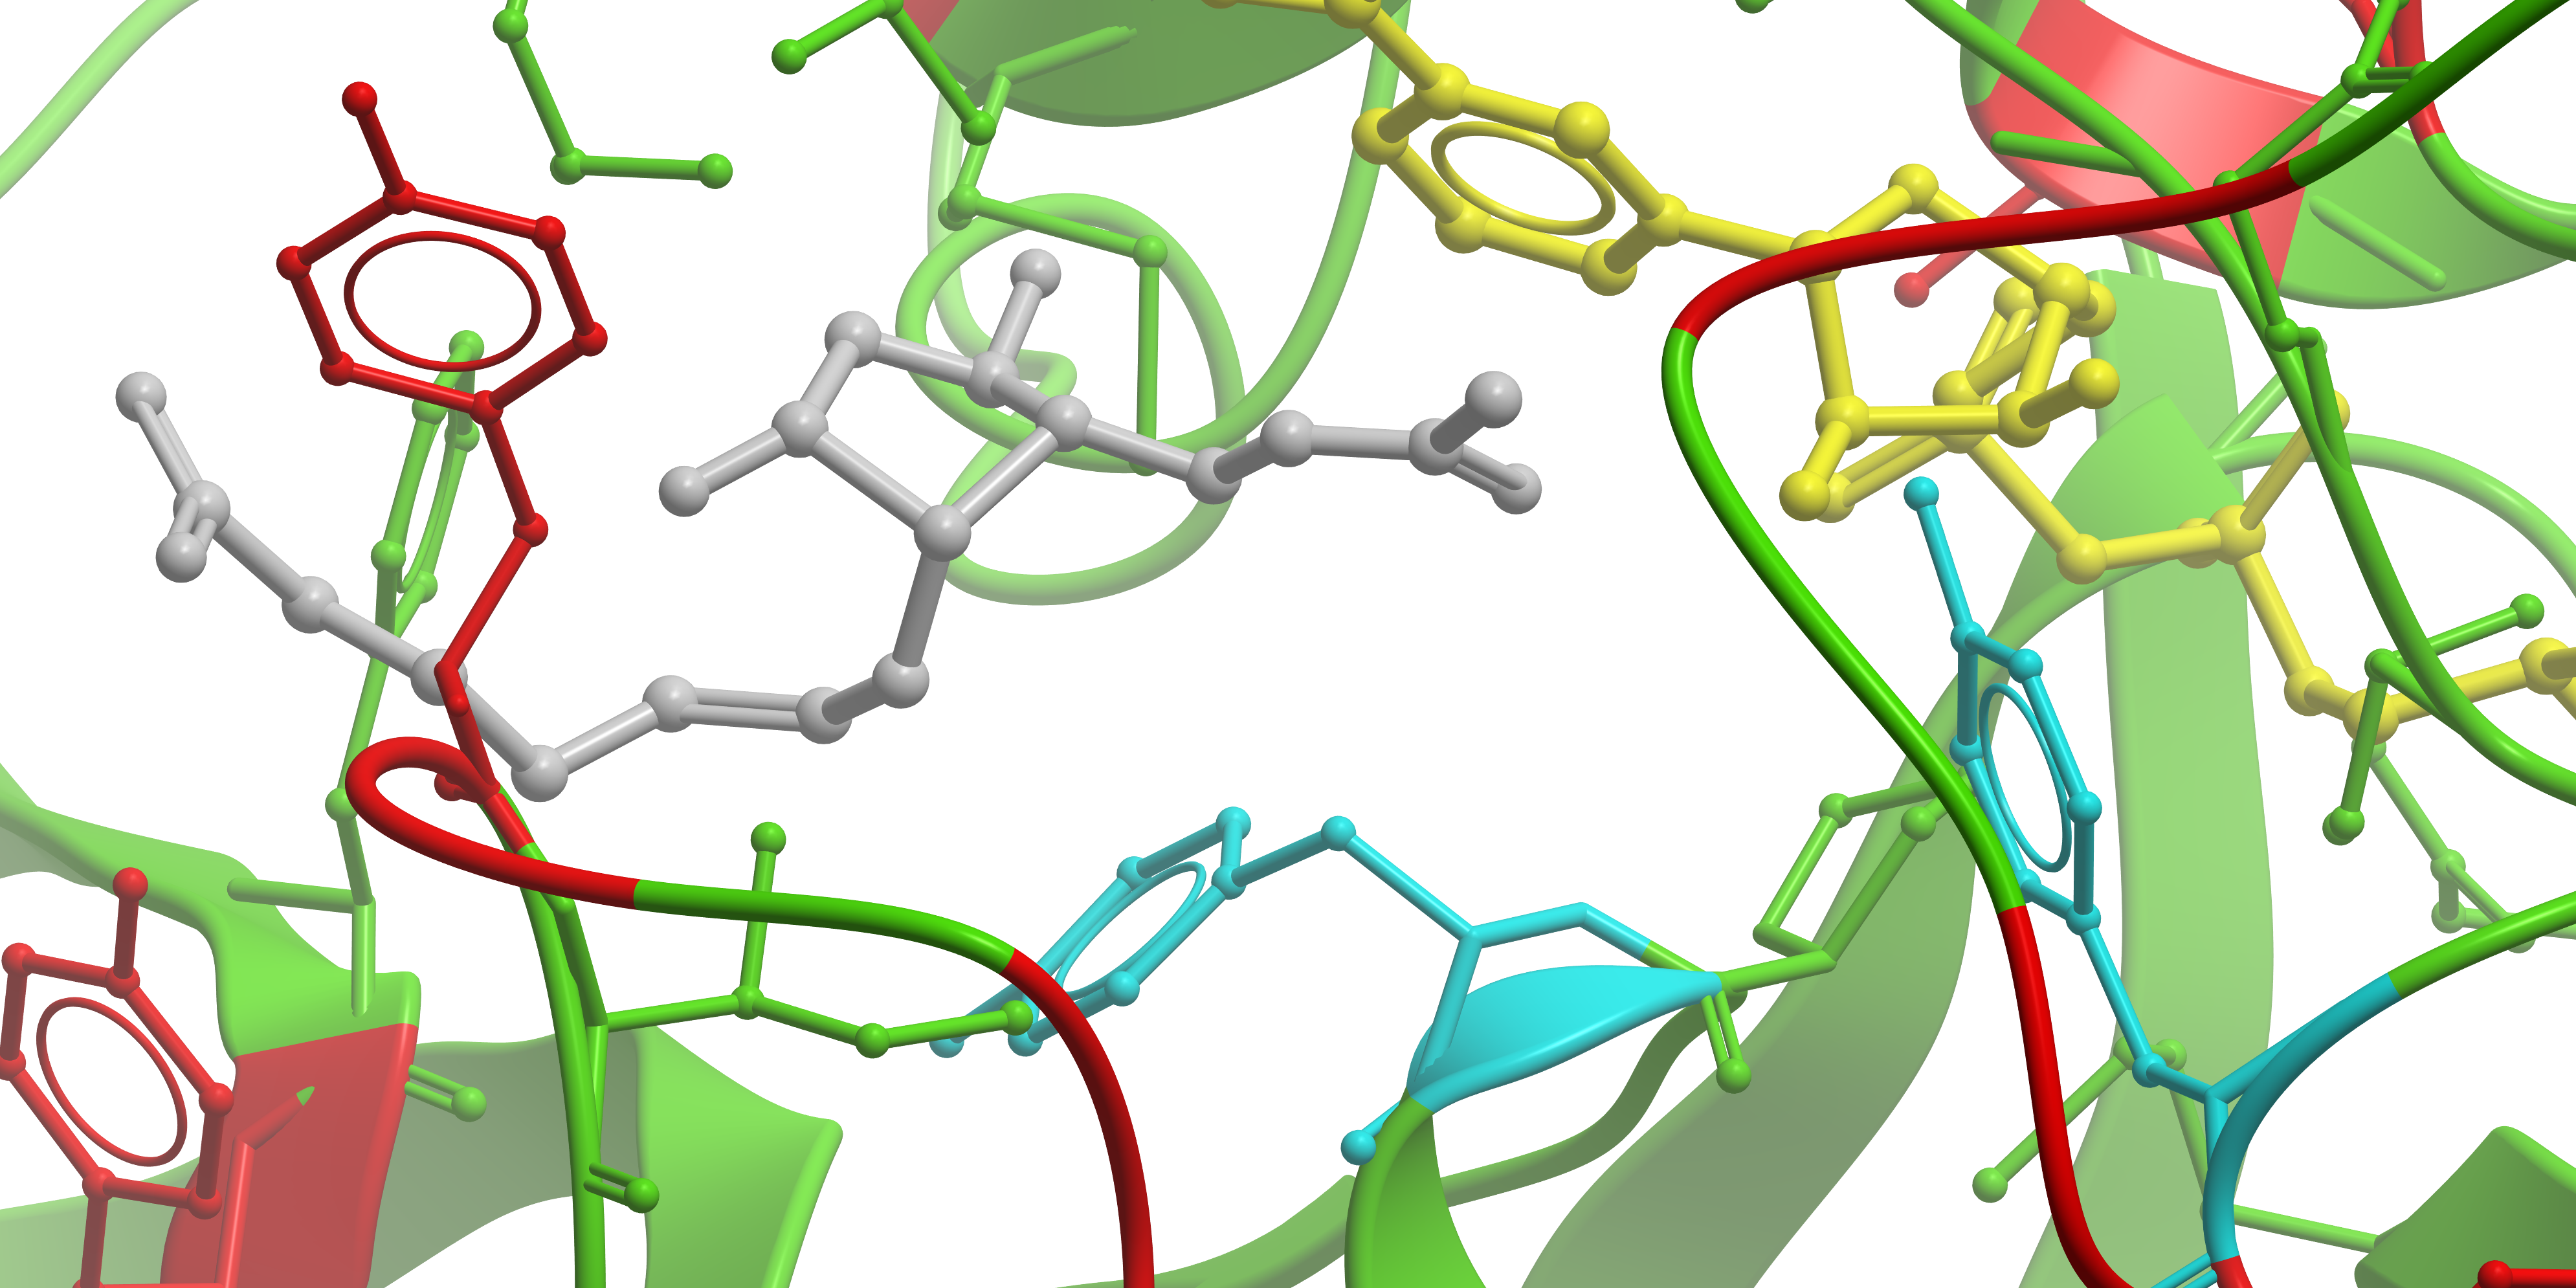
\includegraphics[width=0.89\textwidth]{fig/ptgr2_substrate.png}\\
 {\bf PTGR2}\\
 \vspace{10pt}
 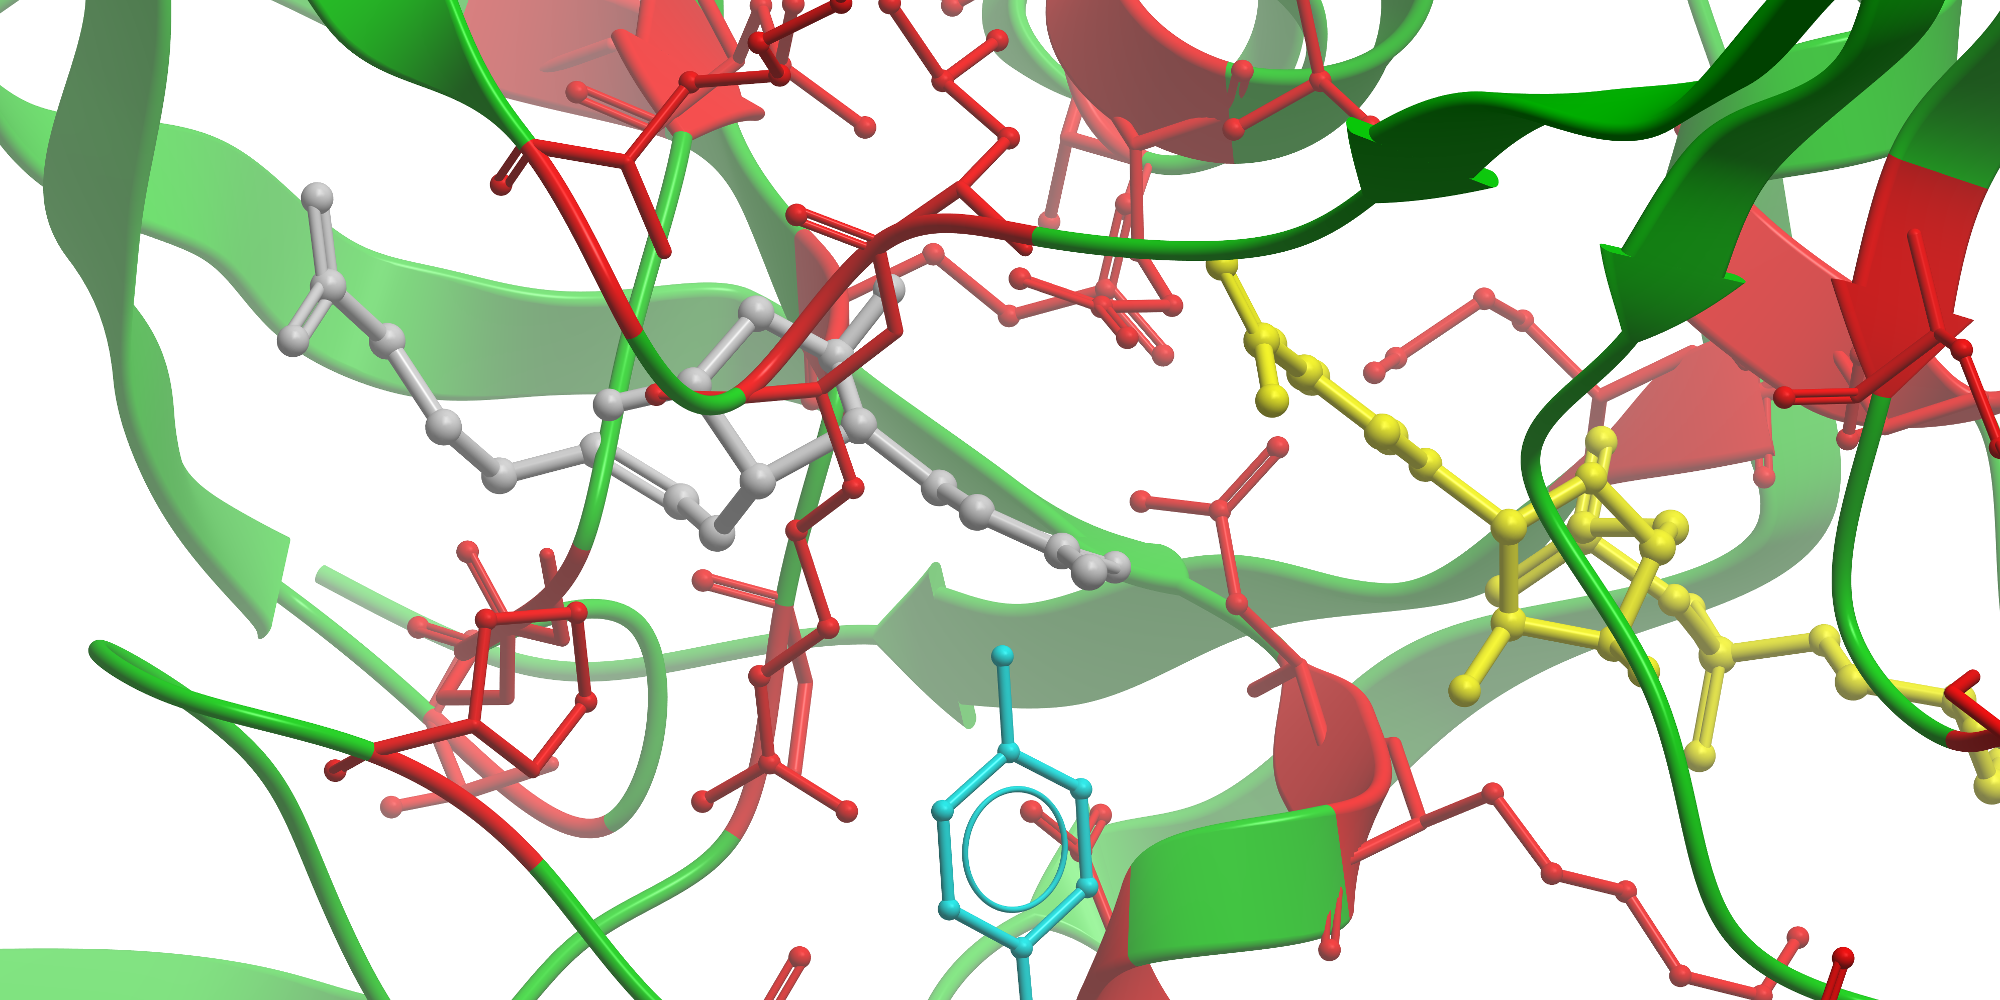
\includegraphics[width=0.89\textwidth]{fig/qorx_substrate.png}\\
 {\bf QORX}\\
 \vspace{10pt}
 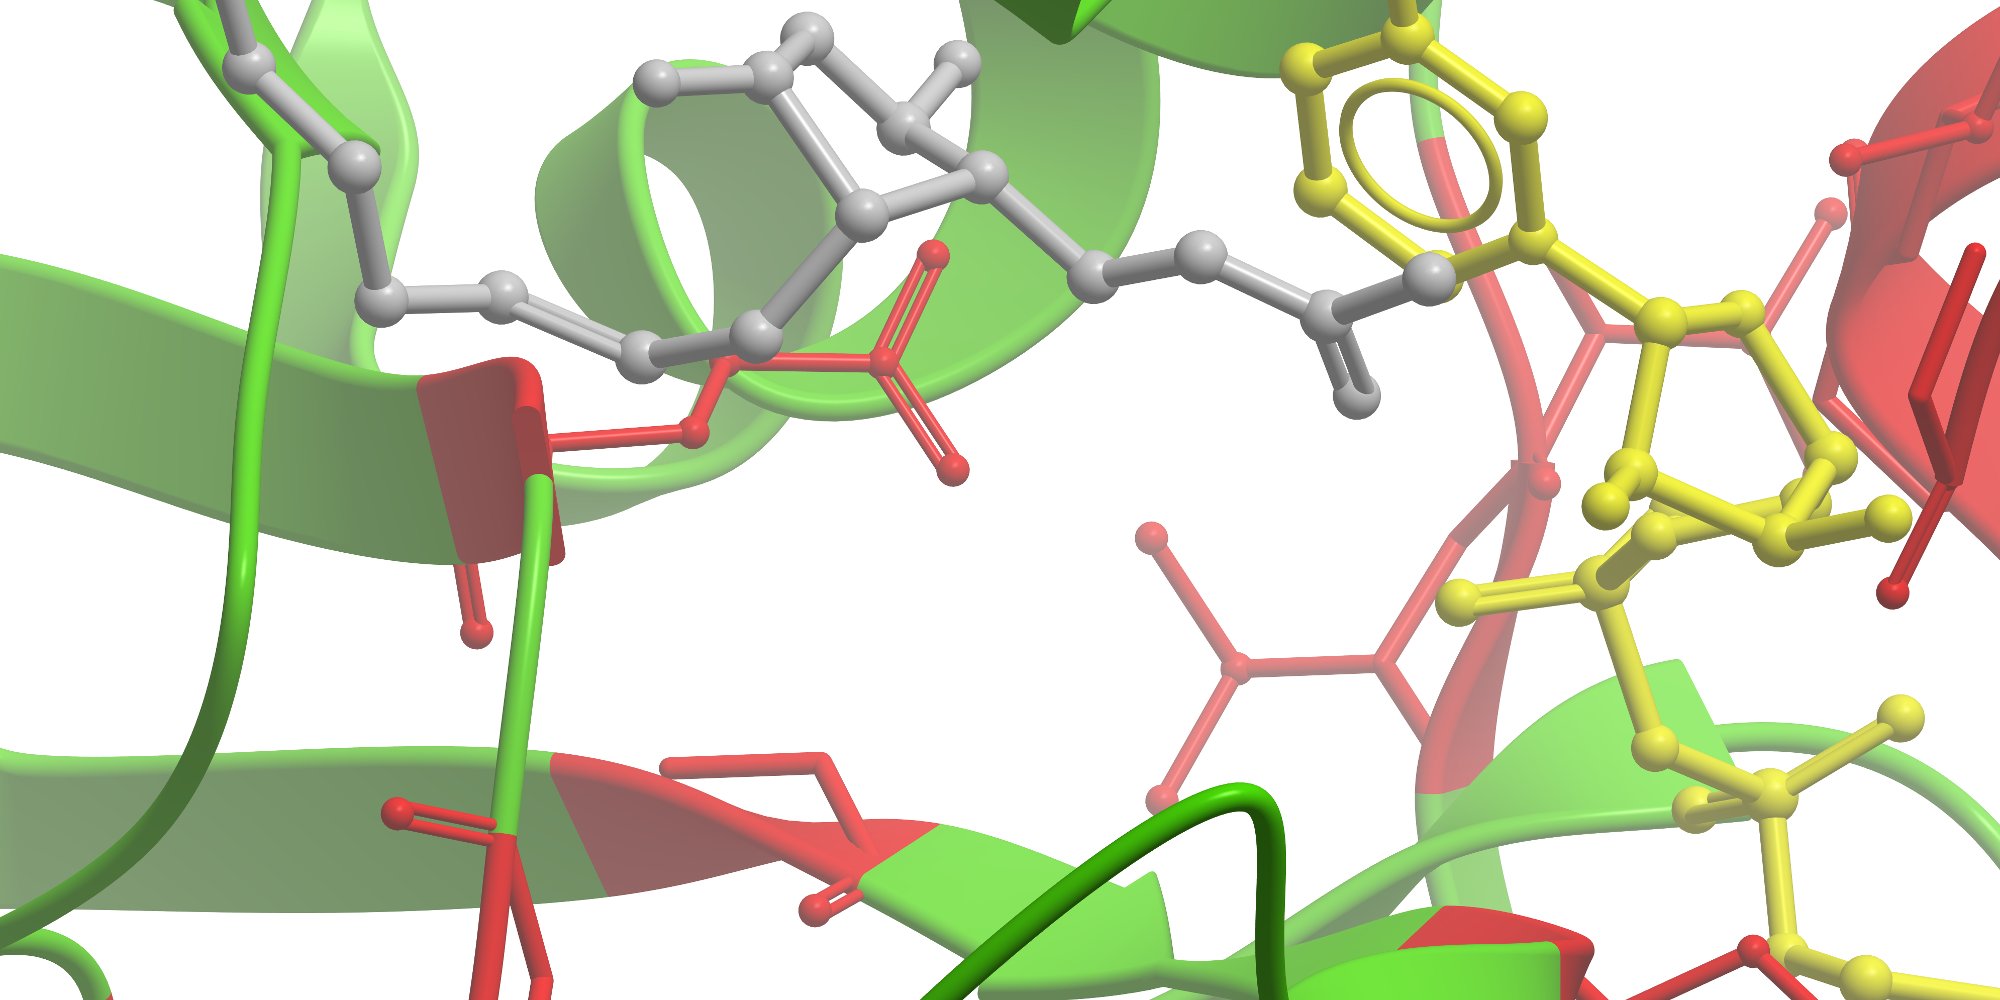
\includegraphics[width=0.89\textwidth]{fig/vat1l_substrate.png}\\
 {\bf VAT1L}\\
 \caption{Substrate binding in the human MDRs. The three identified types use two Tyr (PTGR2; PDB id: 2ZB4), one Tyr (QORX; PDB id: 2J8Z), or neither (VAT1L; PDB id: 4A27). Yellow: NAD(P)H, Gray: substrate, Red: conserved residue, Cyan: Tyr. If a substrate or NAD(P)(H) was missing in the structure, the ones from PTGR2 were used as a reference.}
 \label{fig:mdr_subst_bind}
\end{figure}


\section{Summary}
\label{sec:summary}

The work presented here covered the classification of mammalian ADHs, analysis of mammalian ADH5, and an analysis of the binding pockets of nine MDR members.

An automated strategy was developed to identify new mammalian ADHs that are available in especially the UniProt and NCBI protein databases. Along with this pipeline, an automatic classification system of ADH1--6 was also developed using HMMs. The pipeline was developed in 2014, and the classification is still accurate, as confirmed by phylogenetic trees. As expected, the number of ADH sequences in the databases keep increasing, and there are now 145 mammalian species with at least one known member. The pipeline can thus be used as an automated means of maintaining a database of known mammalian ADHs. It should also be noted that the pipeline allows the correct classification of ADH6, as opposed to the common misclassification of ADH6 proteins as ADH5 or ADH1-like in the sequence databases.

The class V alcohol dehydrogenase, ADH5, has still not been isolated, but the computational analysis imply that there are irregularities in the region for dimer formation, preventing the formation of dimers, which is known to be essential for the stability of mammalian ADHs. Still, there is an evolutionary pressure on the ADH5 genes to maintain their current sequences, and thus the protein should have some function. Taken together, these results imply that ADH5 does not form the traditional homodimers and has a function that differ from that of other ADHs.

The analysis of multiple MDR members showed that there are at least three different types of the substrate-binding part of the binding pockets. Of the proteins that were analysed, most seem to use Tyr to bind substrates, but there was also an example of a proteins that did not use Tyr (VAT1L), and also did not have any other conserved residues that were clear candidates for involvement in substrate binding.

Finally, the work presented here is an excellent example of how research is build on top of earlier work. The development of the pipeline used to identify and classify ADH members could be reused to identify ADH5 members, and with some slight modifications, the code could also be used to identify other MDR members. This is also true for the analysis developed to compare the classes of mammalian ADH while looking for unique residues could be extended and improved for the analysis of other MDRs.


\chapter{General Discussion}
\label{sec:discussion}

The ADH classes are originally defined based on the characteristics of ADH members that have been investigated experimentally\cite{vallee_isozymes_1983, duester_recommended_1999, hoog_mammalian_2001-1}. As a result of this, ADH1--4 are clearly defined and correctly annotated in the databases. As ADH5 has never been isolated in its native form, the available information is very limited, and most ``non-ADH1--4'' sequences have been annotated as ADH5. By aligning and generating phylogenetic trees of the ``ADH5'' protein sequences, it has at multiple occasions, including in paper \ref{paper:mammalian_adhs}, been shown that there is also a sixth class of mammalian ADH. This means that the ADH5 sequence data is easily contaminated by the ADH6 sequence data. Further, a large number of the mammalian ADH sequences that are present in the sequence databases often bear names similar to ``uncharacterized protein'' or ``Alcohol dehydrogenase-like'', making it unclear what class they actually belong to (and if they are ADHs at all).

By developing an automated methodology for the retrieval and classification of ADH sequences, a complete set of all mammalian ADH protein sequences deposited in the major sequence databases could be obtained, and the set can also be kept up to date, being rerun whenever the databases are updated. The retrieved sequences can be used to map the presence of the ADH classes in different species, allowing observations such as the lack of ADH6 in primates, or that ADH5 is a pseudogene in mouse.

BLAST has been used to find homologs of sequences for a long time, including to find new ADHs. The main improvement with the new methodology is the automation, allowing the set of mammalian ADH proteins to be constantly up to date. In addition, the automated classification makes it unnecessary to confirm the classification of e.g. ADH5 proteins manually.

Further, it should be trivial to extend the methodology to cover more classes and other species by just adding new HMM definitions and determining appropriate cutoffs. 

Human ADH5 is the only human ADH that has never been isolated and analysed as a native protein. The work presented here first attempted the isolation of the human and rat ADH5 proteins, but with little success. Fusion proteins were isolated, but they did not display any activity with any of the traditional ADH substrates. The lack of success implies that ADH5 differs greatly from the other human ADHs, as they can all be readily expressed and isolated as native proteins using the same techniques\cite{hoog_mammalian_2001-1} that were used for ADH5.

The fact that ADH5 could be expressed as a fusion protein, but not as a native protein, implies that ADH5 may need a second protein to help stabilise it. The lack of success in isolating the native protein could then be explained by the fact that the needed protein is missing in vitro.

As the protein could not be isolated, the properties were investigated using computational methods instead, attempting to understand why the protein behaved so differently from the other ADHs, even though its sequence was similar. Based on the analysis, there were indications of irregularities in the region involved in the formation of dimers. Further, many highly conserved residues in ADH1--4 were replaced by other residues in ADH5. This could explain the lack of success with the isolation of the protein, as the formation of dimers is known to be important for the stability and function of the other human ADHs\refpaper{paper:adh5_2013}$^,$\cite{hoog_mammalian_2001-1}, fitting the experimental data.

If the ADH5 protein is unstable and has no function, it would be expected that the gene should have many non-synonymous mutations, slowly turning the gene into a pseudogene. This is true in mice, where the ADH5 protein lacks multiple exons \href{https://www.ncbi.nlm.nih.gov/gene/639769}{[NCBI Gene ID: 639769]}. The human ADH5 also has known (albeit rare) mutations of residues that would render the other ADHs unusable. However, an analysis of the evolutionary pressure of ADH5 sequences from multiple species showed that there is no high fraction of non-synonymous mutations, most being synonymous instead. As such, it seems that there is an evolutionary pressure on the ADH5 protein sequence, forcing it to retain its current sequence.

The mouse genome contains two ADH6 genes, and it could be theorised that the function of the ADH5 gene has been overtaken by the one or both of the ADH6 genes. However, rat also has two ADH6 genes, as well as a complete ADH5 gene, making it improbable. There is the possibility that the rat ADH5 is being degraded, though inspection of the protein sequence gives no clear evidence of this, but as the properties of ADH5 are unknown	 it is difficult to evaluate it.

Thus, ADH5 seems to have a function, but it is different from that of other ADHs. It could be that it interacts with another protein in vivo, allowing to perform its effect, but it could also be functioning in a different environment in vivo than what was tested experimentally. The lack of activity could potentially be caused by Lys51, which may cause major changes at the active site, greatly altering the enzyme specificity from that of the other human ADHs, as it replaces a highly conserved His, Thr, or Tyr depending on class\cite{hoog_mammalian_2001-1}. It seems that ADH5 should not be considered a pseudogene, but its function remains unknown.

There are currently 18 proteins identified as MDRs in humans. Of those, seven are the ADHs. Of the remaining eleven, one is SORD, similar to ADH, and one is the complex fatty acid synthase with multiple domains. The remaining nine were analysed at the sequence and structure level, focusing on their binding pockets. The important residues were identified using a combination of residue conservation and the localisation inside the binding pockets. As could be expected, the residues inside the coenzyme part of the binding pocket showed a high level of similarity, implying that all nine should be able to bind NADP(H)\cite{wu_structural_2008}.

The identified residues include most residues that are known to interact with the coenzyme, e.g. Lys178, Tyr193, and AGAVG at position 151--155 (most of the GXGXXG motif\cite{wierenga_prediction_1986}), while e.g. Asn217 and Asn321 (PTGR1 residues/numbering) were missed. Apart from the known residues, the set also included some extra residues, e.g. Met124 and Pro125. These may be of importance for the structure of the coenzyme-binding part of the binding pocket, but do not interact directly with the coenzyme.

The developed methodology identified multiple residues in each of the proteins that were known to be involved in the substrate, but not all. In the case of QORX, only five out of eleven residues that were known to interact\cite{porte_three-dimensional_2009} were identified. In one case, this was due to inter-subunit interactions, the residue interacting with the substrate in the other chain, which could not be identified by the methodology, as it was developed to identify interactions only within a subunit. The remaining residues were mainly overlooked due to limited conservation of the residues in question. It does however mean that the residues that were identified had a greater importance for the general function of each enzyme, rather than the specific interactions needed for only a few species.

The substrate-interacting part of the binding pocket varied between the nine MDRs. Among the nine MDRs, three distinct types were identified. The PTGRs all had two Tyr located in the relevant part of the binding pocket, while the others (with the exception of VAT1L) all had one Tyr. VAT1L was the clear exception, with no conserved residues that are clearly involved in the substrate binding.

The methodology used to evaluate the MDRs with known structure was also used to predict the residues involved in substrate binding in VAT1, showing that it seems to be an enzyme similar to that of QORX and MECR, with similar localisation of the Tyr.

The importance of the Tyr seems to vary between the different MDRs. In PTGR2, it is reported to be involved in the catalytic reaction, though it is not essential\cite{wu_structural_2008}. In QORX, it seems to help with the coordination of the substrate, but mutation of the residue may even increase the catalytic efficiency\cite{porte_three-dimensional_2009}. In the similar MECR protein, mutation of the Tyr causes a near complete loss of function\cite{chen_structural_2008}. Thus, the residue seems to have a large variation in importance, even when its localisation is near identical (as in the case of QORX and MECR), though the function may still be substrate coordination.

The use of Tyr in some MDRs is also similar to what is seen in many SDRs, e.g. the combination of Tyr152, Lys156, and Ser139 first seen in 3-alpha-(or 20-beta)-hydroxysteroid dehydrogenase (P19992)\cite{ghosh_refined_1994}.

Thus, the human MDRs have four distinct mechanisms for substrate binding. The ADHs as well as SORD all have similar mechanisms, involving e.g. a Zn$^{2+}$ ion. The PTGRs use two Tyr, VAT1L a non-defined mechanism, and the remaining MDRs a single Tyr. The involved MDRs are all homologs, but they still have different types of active sites.

The MDR superfamily is interesting from the aspect of evolution. The members vary considerably at the protein sequence level, but their folds are very similar. As noted, there are also multiple different substrate binding types as well as active sites. As an effect of this, the substrate specificity also varies largely. This means that neither the substrate specificity nor catalytic mechanism is conserved within the whole superfamily. Instead, the general fold has been conserved as it allows the binding of NAD(P)(H) as a coenzyme and, it seems, a good starting structure for performing catalysis of the conversion of alcohols and aldehydes. There are also cases where multiple genes have joined together, generating complex enzymes with multiple domains, e.g. fatty acid synthase\cite{jayakumar_human_1995}. Taken together, it is a strong example of the extent that evolution can change the properties of a single gene, over time generating a lot of different effects.

It is very difficult to define the ancestral gene of the MDRs. One suggestion would be ADH3 due to the effect on formaldehyde and/or S-nitrosoglutathione, already considered to be the ancestor of the ADHs\cite{danielsson_enzymogenesis:_1992}\cite{hoog_mammalian_2001-1}. This ADH is present in a very large array of species, both prokaryotes, eukaryotes, and archaea. However, there are many other MDRs that could also fill this role, and the variation at the active sites makes it very complex to evaluate the ancestry.

As has been shown in the work presented here, bioinformatics is a strong complement to experimental biochemical methods. The two fields has a symbiotic relationship, where biochemistry is required to feed the data to bioinformatics, and bioinformatics can in turn perform deeper analysis of the data, generating new hypotheses for the biochemical field.

The work performed on ADH5 is an example of this. The initial in vitro experiments showed that ADH5 could not be easily isolated, and its function could not be evaluated. The use of bioinformatics allowed the construction of a structural model and analysis of the sequence, which in turn led to the hypothesis that ADH5 is unstable due to being unable to form dimers. The addition of the evolutionary pressure analysis then complemented the hypothesis, showing that ADH5 should have some type of function. Thus the final hypothesis, ADH5 not forming dimers, but potentially interacting with something else. This hypothesis could then be tested in vitro, leading back to the field of biochemistry.

The medium-chain dehydrogenase/reductase superfamily is a superfamily that can be found in all phylogenetic branches, both prokaryotic and eukaryotic. The more than 170,000 sequences that are present in UniProt correspond to over 0.2\% of all sequences included in the database. There are 20,199 human proteins in UniProtKB/Swiss-Prot, of which only 18 are MDRs, corresponding to 0.1\%. Thus, it can be expected that at least 1 out of every 1000, and potentially even more than 1 out of every 500, unique protein sequences belong to the MDR superfamily. The work presented here  focused on specific MDRs, but it should be possible to extend the methods to cover more MDRs, and the analysis can give hints to the function of the thousands of MDR proteins that currently have unknown function.


\chapter{Acknowledgements}
\label{sec:acknowledgements}

First of all I would like to thank my supervisors Jan-Olov and Bengt for these valuable and helpful years, including all the help and knowledge they've given me. Mikko should also be included here, as without him I would never have started working with ADHs.

Hans should get a special mention for the collaborations and support.

Petter, Krillot, and Klara for always being ready with help, insults, useless information, or anything else that would or would not fit the situation. Gisela, Josefin, and Harriet for cheering me up when it was needed the most.

Michael, Frank, and Andreas, for being my main company for a long time. It was a sad time when you all finished.

Erik, thanks for all the great times and interesting discussions, and for being a friend since I first ventured into the field of biochemistry and molecular biology.

Anders, thank you for making me interested in molecular biology in the first place.

All the people from my time at MBB. Your help and company has been greatly appreciated. A special thank you goes to Alessandra, who always offered her help with any problems.

Everyone currently or previously at Gamma 6. This also includes all the people I interacted with from other parts of SciLifeLab. It was your presence that made my time here a pleasure.

\begin{otherlanguage*}{russian}
И, наконец, спасибо Наталии и Лине за то, что делаете мою жизнь такой счастливой. Я вас люблю!
\end{otherlanguage*}

\bibliography{zotero}
\bibliographystyle{vancouver}


\end{document}
